% =============================================================================
%  MEG-XL explicado desde cero para neuroingeniería
%  Presentación de seminario (~45 min)
%  Estilo heredado de presentacion_tfm/main.tex
% =============================================================================
\documentclass[aspectratio=169,10pt]{beamer}

\usepackage[utf8]{inputenc}
\usepackage[T1]{fontenc}
\usepackage{lmodern}
\usepackage{textcomp}
% babel-spanish si esta disponible (instalacion completa de TeX Live);
% si no, se recurre a ingles solo para el silabeo, sin tocar el texto.
\newif\ifhasspanishbabel
\IfFileExists{spanish.ldf}{\hasspanishbabeltrue}{\hasspanishbabelfalse}
\ifhasspanishbabel
  \usepackage[spanish,es-tabla]{babel}
\else
  \usepackage[english]{babel}
\fi
\DeclareUnicodeCharacter{00BF}{\textquestiondown}
\DeclareUnicodeCharacter{00A1}{\textexclamdown}
\usepackage{graphicx}
\usepackage{booktabs}
\usepackage{array}
\usepackage{multicol}
\usepackage{amsmath}
\usepackage{amssymb}
\usepackage{pgfpages}
\usepackage{xcolor}
\usepackage{tikz}
\usetikzlibrary{arrows.meta,positioning,fit,calc,shapes.geometric,decorations.pathreplacing,patterns,backgrounds}
\usepackage{hyperref}
\hypersetup{unicode=true}

% Para imprimir las notas del presentador, cambiar a:
% \setbeameroption{show notes on second screen=right}
\setbeameroption{hide notes}

\graphicspath{{figuras/}{../presentacion_tfm/imagenes/}{../memoria/imagenes/}{../memoria/figuras/}{imagenes/}{assets/}}

\usetheme{Madrid}
\usecolortheme{default}
\setbeamertemplate{navigation symbols}{}
\setbeamertemplate{caption}[numbered]
\setbeamerfont{title}{size=\Large,series=\bfseries}
\setbeamerfont{frametitle}{size=\large,series=\bfseries}

\definecolor{deepgreen}{HTML}{0B3D2E}
\definecolor{accent}{HTML}{E76F51}
\definecolor{soft}{HTML}{F1FAEE}
\definecolor{greenish}{HTML}{2A9D8F}
\definecolor{warning}{HTML}{F4A261}
\definecolor{muted}{HTML}{6C757D}
\definecolor{lightgray}{HTML}{F6F7F8}

\definecolor{tfmgreen}{HTML}{0B4A36}
\definecolor{softgreen}{HTML}{EAF5F0}
\definecolor{softred}{HTML}{F9D6CA}
\definecolor{softblue}{HTML}{DDEAF7}
\definecolor{softyellow}{HTML}{FFF0C7}
\definecolor{linegray}{HTML}{6E7D77}

\setbeamercolor{structure}{fg=deepgreen}
\setbeamercolor{palette primary}{fg=white,bg=deepgreen}
\setbeamercolor{palette secondary}{fg=white,bg=deepgreen!85!black}
\setbeamercolor{palette tertiary}{fg=white,bg=deepgreen!70!black}
\setbeamercolor{frametitle}{fg=white,bg=deepgreen}
\setbeamercolor{title}{fg=white,bg=deepgreen}
\setbeamercolor{subtitle}{fg=white}
\setbeamercolor{author}{fg=white}
\setbeamercolor{institute}{fg=white}
\setbeamercolor{date}{fg=white}
\setbeamercolor{title page}{fg=white,bg=deepgreen}
\setbeamercolor{block title}{fg=white,bg=deepgreen}
\setbeamercolor{block body}{fg=black,bg=soft}
\setbeamercolor{block title alerted}{fg=white,bg=accent!85!black}
\setbeamercolor{block body alerted}{fg=black,bg=accent!10}
\setbeamercolor{block title example}{fg=white,bg=greenish!80!black}
\setbeamercolor{block body example}{fg=black,bg=greenish!10}
\setbeamercolor{alerted text}{fg=accent}
\setbeamercolor{section in toc}{fg=deepgreen}

\newcommand{\source}[1]{\vspace{1mm}{\tiny\color{muted}Fuente: #1}}
\newcommand{\bigmetric}[2]{{\huge\bfseries\color{deepgreen}{#1}\par}\vspace{0.8mm}{\scriptsize #2\par}\vspace{3mm}}
\newcommand{\smallmetric}[2]{{\Large\bfseries\color{deepgreen}{#1}\par}{\scriptsize #2\par}}
\newcommand{\term}[1]{\textbf{\color{deepgreen}#1}}
\newcommand{\eng}[1]{{\itshape\color{muted}#1}}

\newlength{\footerlogowidth}
\setlength{\footerlogowidth}{\dimexpr\paperwidth/4-1.5mm\relax}
\newcommand{\footerlogos}{%
  \makebox[\footerlogowidth][c]{\IfFileExists{logo_upv.jpg}{
\includegraphics[height=6mm,keepaspectratio]{logo_upv.jpg}}{}}%
  \makebox[\footerlogowidth][c]{\IfFileExists{logo_miarfid.png}{
\includegraphics[height=6mm,keepaspectratio]{logo_miarfid.png}}{}}%
  \makebox[\footerlogowidth][c]{\IfFileExists{logo_dsiic.png}{\includegraphics[height=6mm,keepaspectratio]{logo_dsiic.png}}{}}%
  \makebox[\footerlogowidth][c]{\IfFileExists{logo_vrain.png}{
\includegraphics[height=5mm,trim=25 115 25 115,clip,keepaspectratio]{logo_vrain.png}}{}}%
}

\setbeamercolor{footer logos}{fg=muted,bg=white}
\setbeamertemplate{footline}{%
  \leavevmode%
  \begin{beamercolorbox}[wd=\paperwidth,ht=7.2mm,dp=1.2mm,leftskip=3mm,rightskip=3mm]{footer logos}%
    \raisebox{-0.3mm}{\footerlogos}%
    \llap{\scriptsize\insertframenumber/\inserttotalframenumber}%
  \end{beamercolorbox}%
}

% --- Estilos TikZ reutilizables -----------------------------------------------
\tikzset{
  blk/.style={draw, rounded corners=3pt, line width=.7pt, fill=white, align=center, inner sep=4pt, font=\scriptsize},
  blkg/.style={blk, fill=softgreen, draw=deepgreen},
  blkb/.style={blk, fill=softblue, draw=deepgreen!60!blue},
  blky/.style={blk, fill=softyellow, draw=warning!80!black},
  blkr/.style={blk, fill=softred, draw=accent!80!black},
  ar/.style={-{Latex[length=2.2mm]}, line width=.8pt, draw=linegray},
  cell/.style={draw=gray!60, line width=.25pt, minimum width=.24cm, minimum height=.20cm, inner sep=0pt},
  lbl/.style={font=\tiny\itshape, text=muted},
}

\title[MEG-XL]{MEG-XL explicado paso a paso}
\subtitle{Cómo un modelo de contexto largo lee palabras en señales cerebrales}
\author{Ricardo Díaz Peris}
\institute{Dpto.\ de Sistemas Informáticos y Computación · UPV}
\date{\today}

\AtBeginSection[]{%
  \begin{frame}[c]{Hoja de ruta}
    \footnotesize
    \tableofcontents[currentsection, hideothersubsections, sectionstyle=show/shaded]
  \end{frame}
}

\begin{document}

% =============================================================================
% 1 — Portada
% =============================================================================
{
\setbeamercolor{background canvas}{bg=deepgreen}
\begin{frame}[plain]
  \vspace{6mm}
  \begin{center}
    {\Large\bfseries\color{white}\inserttitle\par}
    \vspace{3mm}
    {\normalsize\color{white}\insertsubtitle\par}
    \vspace{10mm}
    {\normalsize\color{white}\insertauthor\par}
    \vspace{1.5mm}
    {\small\color{white}\insertinstitute\par}
    \vspace{10mm}
    {\footnotesize\color{white!80}Basado en Jayalath \& Parker Jones (2026), \emph{MEG-XL: Data-Efficient Brain-to-Text\\ via Long-Context Pre-Training}, arXiv:2602.02494\par}
  \end{center}
\end{frame}
}

% =============================================================================
% 2 — Para quién es esta charla
% =============================================================================
\begin{frame}[c]{Qué asumo y qué no asumo}
  \begin{columns}[t,totalwidth=\linewidth]
    \begin{column}{0.48\linewidth}
      \begin{block}{Doy por sabido}
        \small
        \begin{itemize}
          \item Qué es EEG y MEG, y qué mide cada uno.
          \item Filtrado, remuestreo, Nyquist, artefactos.
          \item Media, varianza, producto escalar, matrices.
          \item Que una señal cerebral tiene muy poca relación señal-ruido.
        \end{itemize}
      \end{block}
    \end{column}
    \begin{column}{0.48\linewidth}
      \begin{alertblock}{NO doy por sabido}
        \small
        \begin{itemize}
          \item Qué es un \eng{transformer}.
          \item Qué es la \eng{atención}, un \eng{token} o un \eng{embedding}.
          \item Qué significa preentrenar o ajustar un modelo.
          \item Nada de jerga de aprendizaje profundo.
        \end{itemize}
      \end{alertblock}
    \end{column}
  \end{columns}
  \vspace{3mm}
  \centering\small
  Cada término nuevo aparece \term{marcado} la primera vez y se explica con vocabulario de procesado de señal.
  \note{Aviso inicial: voy despacio en la parte 2 (vocabulario). Si alguien ya sabe qué es atención, la parte 3 es la interesante.}
\end{frame}

% =============================================================================
% 3 — Índice
% =============================================================================
\begin{frame}[c]{Hoja de ruta}
  \footnotesize
  \tableofcontents
\end{frame}

% #############################################################################
\section{El problema: leer palabras del cerebro}
% #############################################################################

% --- 4 ---
\begin{frame}[c]{El objetivo: \emph{brain-to-text} no invasivo}
  \centering
  \resizebox{0.95\textwidth}{!}{%
  \begin{tikzpicture}[node distance=6mm]
    \node[blkb, minimum height=1.3cm, minimum width=2.4cm] (est) {Estímulo\\ \scriptsize``the fruit bowl\\had a pineapple''};
    \node[blkg, right=10mm of est, minimum height=1.3cm, minimum width=2.4cm] (cer) {Cerebro\\ \scriptsize respuesta neural\\distribuida};
    \node[blky, right=10mm of cer, minimum height=1.3cm, minimum width=2.4cm] (sen) {Sensores\\ \scriptsize 306 canales MEG\\ a 1000\,Hz};
    \node[blkr, right=10mm of sen, minimum height=1.3cm, minimum width=2.4cm] (mod) {Modelo\\ \scriptsize MEG-XL};
    \node[blk, right=10mm of mod, minimum height=1.3cm, minimum width=2.4cm, fill=softgreen] (out) {Texto\\ \scriptsize ``\ldots pineapple''};
    \draw[ar] (est) -- (cer);
    \draw[ar] (cer) -- (sen);
    \draw[ar] (sen) -- (mod);
    \draw[ar] (mod) -- (out);
    \node[lbl, below=1mm of cer] {física};
    \node[lbl, below=1mm of sen] {instrumentación};
    \node[lbl, below=1mm of mod] {esta charla};
  \end{tikzpicture}}

  \vspace{5mm}
  \small
  \begin{itemize}
    \item La aplicación clínica objetivo: pacientes con parálisis o síndrome de enclaustramiento que \term{no pueden hablar}.
    \item No invasivo (MEG/EEG) evita la craneotomía, el tejido cicatricial y el reemplazo quirúrgico del implante.
    \item Precio a pagar: la relación señal-ruido es \term{órdenes de magnitud peor} que con electrodos intracraneales.
  \end{itemize}
  \note{Insistir: MEG-XL decodifica habla PERCIBIDA (el sujeto escucha), no habla imaginada. Es un paso previo.}
\end{frame}

% --- 5 ---
\begin{frame}[c]{El cuello de botella no es el modelo: son los datos por sujeto}
  \footnotesize
  \begin{columns}[T,totalwidth=\linewidth]
    \begin{column}{0.52\linewidth}
      \begin{itemize}
        \item El estado del arte supervisado (d'Ascoli et al., 2025) funciona, pero necesita \term{decenas de horas de grabación del mismo sujeto}.
        \item Sus análisis muestran que importan más las \term{horas por sujeto} que las horas totales.
        \item Un paciente con ELA no puede pasar 50 horas en un MEG.
      \end{itemize}
      \vspace{1mm}
      \begin{alertblock}{La pregunta}
        ¿Se puede sustituir ``muchas horas de \emph{este} sujeto'' por ``muchas horas de \emph{otros} sujetos''?
      \end{alertblock}
    \end{column}
    \begin{column}{0.44\linewidth}
      \centering
      \resizebox{\linewidth}{!}{%
      \begin{tikzpicture}
        \draw[ar] (0,0) -- (6.4,0) node[right, font=\scriptsize] {horas/sujeto};
        \draw[ar] (0,0) -- (0,3.6) node[above, font=\scriptsize] {precisión};
        \draw[draw=accent, line width=1.1pt] (0.2,0.35) .. controls (2,0.6) and (3,2.2) .. (6,3.1);
        \node[font=\scriptsize, text=accent, anchor=west] at (3.4,1.55) {supervisado};
        \draw[draw=deepgreen, line width=1.1pt] (0.2,1.5) .. controls (1.6,2.5) and (3,2.75) .. (6,2.95);
        \node[font=\scriptsize, text=deepgreen, anchor=west] at (1.1,2.9) {preentrenado};
        \draw[dashed, gray] (1.55,0) -- (1.55,3.3);
        \node[font=\scriptsize, text=muted, align=center, anchor=north] at (1.55,-0.15) {régimen\\clínico};
      \end{tikzpicture}}
      \vspace{1mm}
      {\tiny\color{muted}Esquema conceptual de la Figura 3 del artículo.}
    \end{column}
  \end{columns}
\end{frame}

% --- 6 ---
\begin{frame}[c]{La segunda idea: nadie estaba mirando suficiente señal a la vez}
  \small
  \begin{itemize}
    \item Los decodificadores clásicos recortan ventanas del \term{tamaño de la unidad que quieren decodificar}: 0{,}5--3\,s para un fonema, sílaba o palabra.
    \item Eso asume implícitamente que \term{la información relevante es local}.
    \item Pero el habla tiene estructura a escalas mucho mayores: fonemas $\rightarrow$ sílabas $\rightarrow$ palabras $\rightarrow$ frases $\rightarrow$ discurso. Y la señal además arrastra estructura del sujeto, del ruido y del equipo.
  \end{itemize}
  \vspace{2mm}
  \begin{center}
  \resizebox{0.9\textwidth}{!}{%
  \begin{tikzpicture}
    \draw[line width=.8pt, draw=linegray] (0,0) -- (13,0);
    \foreach \x in {0,...,25}{ \draw[draw=gray!50] (\x*0.52,-0.12) -- (\x*0.52,0.12); }
    \node[lbl, below=2mm of {(6.5,0)}] {150 segundos de MEG continuo};
    \draw[draw=accent, line width=1pt, fill=accent!15] (2.0,-0.45) rectangle (2.55,0.45);
    \node[font=\scriptsize, text=accent, anchor=south] at (2.3,0.55) {enfoque clásico: 3\,s};
    \draw[draw=deepgreen, line width=1pt, fill=deepgreen!10, rounded corners=2pt] (0,-0.9) rectangle (13,-0.55);
    \node[font=\scriptsize, text=deepgreen, anchor=north] at (6.5,-0.95) {MEG-XL: 2,5 minutos completos = 5--300$\times$ más contexto que el trabajo previo};
  \end{tikzpicture}}
  \end{center}
  \note{Analogía: es como intentar entender una conversación oyendo sólo palabras sueltas de 3 segundos, sin las anteriores.}
\end{frame}

% --- 7 ---
\begin{frame}[c]{MEG-XL en una diapositiva}
  \small
  \begin{block}{Idea}
    Preentrenar un modelo con \term{muestras de 2,5 minutos de MEG continuo}, sin etiquetas, tapando trozos de señal y obligándolo a reconstruirlos. Después, ajustarlo a la tarea de decodificar palabras con muy pocos datos etiquetados.
  \end{block}
  \vspace{1mm}
  \begin{columns}[c,totalwidth=\linewidth]
    \begin{column}{0.24\linewidth}\centering\bigmetric{150\,s}{contexto por muestra}\end{column}
    \begin{column}{0.24\linewidth}\centering\bigmetric{191k}{posiciones de entrada}\end{column}
    \begin{column}{0.24\linewidth}\centering\bigmetric{20M}{parámetros (vs 200M del supervisado)}\end{column}
    \begin{column}{0.24\linewidth}\centering\bigmetric{$\sim$300\,h}{MEG de $>$800 sujetos}\end{column}
  \end{columns}
  \vspace{1mm}
  \begin{exampleblock}{Resultado}
    Con el 13\,\% de los datos de ajuste: 47--57\,\% de acierto Top-10 frente al 20\,\% del azar, mientras que el resto de modelos fundacionales se quedan al nivel del azar.
  \end{exampleblock}
  \note{Esta diapositiva es el resumen ejecutivo. Si alguien se duerme a partir de aquí, ya sabe el mensaje.}
\end{frame}

% #############################################################################
\section{Vocabulario mínimo: qué es un transformer}
% #############################################################################

% --- 8 ---
\begin{frame}[c]{Una red neuronal es una función con mandos ajustables}
  \small
  \begin{columns}[c,totalwidth=\linewidth]
    \begin{column}{0.52\linewidth}
      Una \term{capa} de red neuronal hace exactamente esto:
      \[ \mathbf{y} = f(W\mathbf{x} + \mathbf{b}) \]
      \begin{itemize}
        \item $\mathbf{x}$: vector de entrada (por ejemplo, 512 números).
        \item $W$: matriz de \term{pesos}. Es un banco de filtros lineales: cada fila calcula un producto escalar con la entrada.
        \item $f$: una no linealidad (aquí, \term{SELU}); sin ella, apilar capas no añadiría nada, porque la composición de funciones lineales es lineal.
        \item \term{Parámetros} $=$ los números de $W$ y $\mathbf{b}$. MEG-XL tiene 20 millones.
      \end{itemize}
    \end{column}
    \begin{column}{0.44\linewidth}
      \centering
      \resizebox{\linewidth}{!}{%
      \begin{tikzpicture}
        \foreach \y in {0,1,2,3}{ \node[circle, draw=deepgreen, fill=softgreen, minimum size=5.5mm, inner sep=0] (i\y) at (0,\y*0.85) {}; }
        \foreach \y in {0,1,2}{ \node[circle, draw=warning!80!black, fill=softyellow, minimum size=5.5mm, inner sep=0] (h\y) at (2.4,\y*0.85+0.42) {}; }
        \foreach \y in {0,1}{ \node[circle, draw=accent!80!black, fill=softred, minimum size=5.5mm, inner sep=0] (o\y) at (4.8,\y*0.85+0.85) {}; }
        \foreach \a in {0,1,2,3}{\foreach \b in {0,1,2}{ \draw[draw=gray!45, line width=.3pt] (i\a) -- (h\b); }}
        \foreach \a in {0,1,2}{\foreach \b in {0,1}{ \draw[draw=gray!45, line width=.3pt] (h\a) -- (o\b); }}
        \node[font=\scriptsize, below=1mm of i0] {entrada $\mathbf{x}$};
        \node[font=\scriptsize, below=2mm of h0] {$f(W_1\mathbf{x}+\mathbf{b}_1)$};
        \node[font=\scriptsize, below=4mm of o0] {salida $\mathbf{y}$};
      \end{tikzpicture}}
    \end{column}
  \end{columns}
  \note{Analogía útil: W es un banco de filtros FIR, pero cuyos coeficientes se aprenden en lugar de diseñarse.}
\end{frame}

% --- 9 ---
\begin{frame}[c]{Vector de características (\eng{embedding})}
  \small
  \begin{block}{Definición operativa}
    Un \term{embedding} es simplemente un \term{vector de $d$ números reales} que representa un objeto (un instante de señal, una palabra, un sensor). Nada más.
  \end{block}
  \vspace{2mm}
  \begin{columns}[t,totalwidth=\linewidth]
    \begin{column}{0.5\linewidth}
      \textbf{Lo que ya conoces con otro nombre:}
      \begin{itemize}
        \item El vector de potencias por banda $(\delta,\theta,\alpha,\beta,\gamma)$ de una época es un embedding de dimensión 5.
        \item Los coeficientes MFCC de una trama de voz son un embedding.
        \item La diferencia: aquí las componentes no las diseñas tú, las \term{aprende el modelo}.
      \end{itemize}
    \end{column}
    \begin{column}{0.5\linewidth}
      \textbf{Por qué importa la geometría:}
      \begin{itemize}
        \item Si dos objetos son parecidos, sus vectores apuntan en direcciones parecidas.
        \item Se mide con la \term{similitud coseno}:
        \[ \cos(\mathbf{u},\mathbf{v}) = \frac{\mathbf{u}\cdot\mathbf{v}}{\|\mathbf{u}\|\,\|\mathbf{v}\|} \]
        \item Esto será literalmente el criterio de decisión final del sistema.
      \end{itemize}
    \end{column}
  \end{columns}
  \vspace{2mm}
  \centering
  {\footnotesize En MEG-XL, $d_{\text{model}} = 512$: cada instante de cada sensor se describe con 512 números.}
\end{frame}

% --- 10 ---
\begin{frame}[c]{Entrenar $=$ bajar una pendiente}
  \small
  \begin{columns}[c,totalwidth=\linewidth]
    \begin{column}{0.54\linewidth}
      \begin{enumerate}
        \item Se define una \term{función de pérdida} $\mathcal{L}$: un número que mide cuánto se equivoca el modelo.
        \item Se calcula el \term{gradiente} $\partial\mathcal{L}/\partial W$: en qué dirección habría que mover cada parámetro para que la pérdida baje.
        \item Se da un pasito en esa dirección: $W \leftarrow W - \eta\,\partial\mathcal{L}/\partial W$. La \term{tasa de aprendizaje} $\eta$ es el tamaño del paso ($10^{-4}$ en el preentrenamiento).
        \item Se repite. MEG-XL da \term{35\,000 pasos}, unas 12 horas en una GPU H100.
      \end{enumerate}
      \vspace{1mm}
      {\footnotesize El optimizador concreto es \term{AdamW}: gradiente descendente con memoria del paso anterior y decaimiento de pesos.}
    \end{column}
    \begin{column}{0.42\linewidth}
      \centering
      \resizebox{\linewidth}{!}{%
      \begin{tikzpicture}
        \draw[ar] (-0.3,0) -- (6.2,0) node[right, font=\scriptsize] {parámetro};
        \draw[ar] (0,-0.3) -- (0,3.4) node[above, font=\scriptsize] {pérdida $\mathcal{L}$};
        \draw[draw=deepgreen, line width=1.2pt] plot[domain=0.3:5.7, samples=60] (\x, {0.35+0.32*(\x-3)*(\x-3)});
        \foreach \x/\lab in {5.2/, 4.4/, 3.7/, 3.25/}{
          \filldraw[accent] (\x, {0.35+0.32*(\x-3)*(\x-3)}) circle (2.1pt);
        }
        \draw[-{Latex[length=1.8mm]}, accent, line width=.8pt] (5.2,{0.35+0.32*4.84}) -- (4.45,{0.35+0.32*1.96});
        \draw[-{Latex[length=1.8mm]}, accent, line width=.8pt] (4.4,{0.35+0.32*1.96}) -- (3.75,{0.35+0.32*0.49});
        \node[font=\scriptsize, text=accent, anchor=west] at (4.6,2.6) {cada paso};
        \filldraw[deepgreen] (3,0.35) circle (2.4pt) node[below, font=\scriptsize] {mínimo};
      \end{tikzpicture}}
    \end{column}
  \end{columns}
\end{frame}

% --- 11 ---
\begin{frame}[c]{Preentrenar y ajustar: la analogía del residente}
  \small
  \begin{columns}[t,totalwidth=\linewidth]
    \begin{column}{0.48\linewidth}
      \begin{block}{Fase 1: preentrenamiento (\eng{pre-training})}
        \begin{itemize}
          \item Se usan \term{muchísimos datos sin etiquetar}: 300 h de MEG de más de 800 sujetos, en reposo, tareas motoras y de lenguaje.
          \item No hay ninguna palabra que predecir todavía.
          \item El modelo aprende ``cómo es una señal MEG normal'': qué ocurre a la vez en sensores vecinos, qué ritmos se encadenan, cómo evoluciona todo en el tiempo.
        \end{itemize}
      \end{block}
    \end{column}
    \begin{column}{0.48\linewidth}
      \begin{exampleblock}{Fase 2: ajuste fino (\eng{fine-tuning})}
        \begin{itemize}
          \item Se usan \term{pocos datos etiquetados}: grabaciones con las palabras marcadas en el tiempo.
          \item Se parte de los pesos ya aprendidos y se retocan suavemente (tasa de aprendizaje $10^{-5}$, 100 veces menor).
          \item Es el residente que ya lleva años viendo trazados y ahora sólo aprende a marcar una patología concreta.
        \end{itemize}
      \end{exampleblock}
    \end{column}
  \end{columns}
  \vspace{2mm}
  \centering\small
  \term{Hipótesis central del artículo:} los priores aprendidos en la fase 1 sustituyen a las horas de grabación del sujeto en la fase 2.
  \note{Esta es la diapositiva que hay que dejar clara antes de entrar en la arquitectura. Todo lo demás es maquinaria para hacer esto posible.}
\end{frame}

% --- 12 ---
\begin{frame}[c]{Aprendizaje autosupervisado: tapar y adivinar}
  \small
  \begin{columns}[c,totalwidth=\linewidth]
    \begin{column}{0.46\linewidth}
      \begin{itemize}
        \item \term{Supervisado}: te doy señal y te doy la respuesta correcta (la palabra). Caro: hay que grabar con estímulos anotados.
        \item \term{Autosupervisado}: la propia señal genera su etiqueta. Tapo un trozo y la etiqueta es \emph{lo que había ahí}.
        \item Coste de etiquetado: cero. Se puede usar cualquier grabación MEG existente.
        \item Para acertar lo tapado, el modelo tiene que haber aprendido la estructura real de la señal.
      \end{itemize}
    \end{column}
    \begin{column}{0.5\linewidth}
      \centering
      \resizebox{\linewidth}{!}{%
      \begin{tikzpicture}
        \foreach \c in {0,...,5}{
          \foreach \t in {0,...,23}{
            \pgfmathtruncatemacro{\mask}{ (\t>6 && \t<11) || (\t>16 && \t<20) ? 1 : 0}
            \ifnum\mask=1
              \draw[cell, fill=accent!35, draw=accent!70!black] (\t*0.28,\c*0.26) rectangle ++(0.28,0.26);
            \else
              \pgfmathtruncatemacro{\m}{mod(\t+2*\c,4)}
              \ifnum\m=0 \def\col{deepgreen!12}\fi
              \ifnum\m=1 \def\col{deepgreen!25}\fi
              \ifnum\m=2 \def\col{deepgreen!8}\fi
              \ifnum\m=3 \def\col{deepgreen!18}\fi
              \draw[cell, fill=\col] (\t*0.28,\c*0.26) rectangle ++(0.28,0.26);
            \fi
          }
        }
        \node[rotate=90, font=\scriptsize, anchor=south] at (-0.25,0.78) {sensores};
        \node[font=\scriptsize] at (3.36,-0.35) {tiempo};
        \node[font=\scriptsize, text=accent, anchor=west] at (7.0,1.3) {tapado};
        \node[font=\scriptsize, text=deepgreen, anchor=west] at (7.0,0.6) {visible};
        \draw[ar, accent] (6.9,1.3) -- (5.6,1.3);
      \end{tikzpicture}}
      \vspace{1mm}
      {\tiny\color{muted}El modelo debe reconstruir las columnas naranjas usando sólo lo verde.}
    \end{column}
  \end{columns}
\end{frame}

% --- 13 ---
\begin{frame}[c]{¿Qué es un \eng{token}?}
  \small
  \begin{block}{En texto}
    Un \term{token} es un trocito de texto convertido en un \term{símbolo de un catálogo finito}. ``pineapple'' $\rightarrow$ token \#4412 de un vocabulario de, digamos, 32\,000 símbolos.
  \end{block}
  \vspace{1mm}
  \begin{alertblock}{El problema en señales biológicas}
    El MEG es \term{continuo}. No hay ningún catálogo natural de símbolos. Hay que \term{fabricarlo}.
  \end{alertblock}
  \vspace{1mm}
  \textbf{¿Por qué molestarse en discretizar?} Dos razones muy concretas:
  \begin{enumerate}
    \item \term{Da un objetivo de entrenamiento bien definido.} Predecir un símbolo de entre 256 es un problema de clasificación con una pérdida estándar (entropía cruzada). Predecir un valor continuo obligaría a elegir una métrica de error en amplitud, dominada por el ruido.
    \item \term{Comprime.} El tokenizador reduce el eje temporal por un factor $r = 12$. Sin esa compresión, la ventana de 150\,s no cabe en la memoria de la GPU.
  \end{enumerate}
  \note{Si preguntan: sí, se podría hacer regresión sobre la señal cruda; el artículo elige tokens por SoundStorm/wav2vec y porque comprime.}
\end{frame}

% --- 14 ---
\begin{frame}[c]{Atención (1/3): el problema que resuelve}
  \small
  Tenemos una secuencia de 625 vectores (uno por instante). Queremos que cada instante se \term{enriquezca con información de los demás}, pero:
  \begin{itemize}
    \item No sabemos de antemano \term{cuáles} son los instantes relevantes. Depende del contenido de la señal.
    \item Un filtro FIR clásico usa \term{pesos fijos} sobre una vecindad fija.
  \end{itemize}
  \vspace{2mm}
  \begin{block}{Atención, en una frase}
    Un \term{promedio ponderado en el que los pesos se calculan a partir de los propios datos}, en cada posición y en cada pasada.
  \end{block}
  \vspace{2mm}
  \centering
  \resizebox{0.86\textwidth}{!}{%
  \begin{tikzpicture}
    \node[font=\scriptsize\bfseries, anchor=west] at (0,2.2) {Filtro FIR};
    \foreach \i/\w in {0/0.15,1/0.35,2/0.8,3/0.35,4/0.15}{
      \draw[fill=muted!30, draw=muted] (\i*0.7,1.1) rectangle ++(0.5,\w*1.2);
    }
    \node[font=\tiny, text=muted, anchor=north, align=center] at (1.75,1.0) {coeficientes fijos,\\iguales para toda la señal};

    \node[font=\scriptsize\bfseries, anchor=west] at (6.5,2.2) {Atención};
    \foreach \i/\w in {0/0.1,1/0.75,2/0.2,3/0.1,4/0.6}{
      \draw[fill=deepgreen!45, draw=deepgreen] (6.5+\i*0.7,1.1) rectangle ++(0.5,\w*1.2);
    }
    \node[font=\tiny, text=deepgreen, anchor=north, align=center] at (8.25,1.0) {pesos recalculados para cada posición,\\a partir del contenido de la señal};
    \draw[ar, line width=1pt] (4.3,1.5) -- (6.2,1.5);
  \end{tikzpicture}}
\end{frame}

% --- 15 ---
\begin{frame}[c]{Atención (2/3): consulta, clave y valor}
  \small
  Cada vector de entrada $\mathbf{h}_t$ se proyecta con tres matrices aprendidas y produce tres vectores distintos:
  \vspace{1mm}
  \begin{columns}[t,totalwidth=\linewidth]
    \begin{column}{0.32\linewidth}
      \begin{block}{Consulta $\mathbf{q}_t = W_Q\mathbf{h}_t$}
        \scriptsize ``Qué tipo de información estoy buscando.''
      \end{block}
    \end{column}
    \begin{column}{0.32\linewidth}
      \begin{block}{Clave $\mathbf{k}_t = W_K\mathbf{h}_t$}
        \scriptsize ``Qué tipo de información ofrezco yo.''
      \end{block}
    \end{column}
    \begin{column}{0.32\linewidth}
      \begin{block}{Valor $\mathbf{v}_t = W_V\mathbf{h}_t$}
        \scriptsize ``El contenido que entrego si me eligen.''
      \end{block}
    \end{column}
  \end{columns}
  \vspace{3mm}
  El peso que la posición $t$ da a la posición $k$ es la \term{similitud entre la consulta de $t$ y la clave de $k$}, normalizada:
  \[
    A_{t,k} = \frac{\exp\!\big(\mathbf{q}_t\cdot\mathbf{k}_k/\sqrt{d}\big)}{\sum_{j}\exp\!\big(\mathbf{q}_t\cdot\mathbf{k}_j/\sqrt{d}\big)}
    \qquad\Longrightarrow\qquad
    \mathbf{z}_t = \sum_k A_{t,k}\,\mathbf{v}_k
  \]
  \vspace{1mm}
  \begin{itemize}\scriptsize
    \item El producto escalar $\mathbf{q}_t\cdot\mathbf{k}_k$ es un \term{detector de coincidencia}: grande si ambos vectores apuntan en la misma dirección. Es, literalmente, una correlación.
    \item La división por $\sqrt{d}$ evita que los productos escalares crezcan con la dimensión y saturen la exponencial.
    \item La \term{softmax} (exponencial normalizada) fuerza que los pesos sean positivos y sumen 1: es un promedio ponderado honesto.
  \end{itemize}
  \note{Insistir en que A es una matriz de pesos de promediado, fila a fila suma 1. Nada mágico.}
\end{frame}

% --- 16 ---
\begin{frame}[c]{Atención (3/3): qué sale de ahí, visualmente}
  \centering
  \resizebox{0.78\textwidth}{!}{%
  \begin{tikzpicture}
    % secuencia
    \foreach \i in {0,...,7}{
      \node[blk, minimum width=0.85cm, minimum height=0.55cm] (h\i) at (\i*1.15,0) {$\mathbf{h}_{\i}$};
    }
    \node[blkr, minimum width=0.85cm, minimum height=0.55cm] at (3*1.15,0) {$\mathbf{h}_{3}$};
    \node[lbl, below=1mm of h0] {instante 0};
    \node[lbl, below=1mm of h7] {instante 7};

    % pesos
    \foreach \i/\w in {0/0.10,1/0.05,2/0.30,3/0.15,4/0.05,5/0.05,6/0.25,7/0.05}{
      \draw[draw=deepgreen, fill=deepgreen!45, line width=.4pt] (\i*1.15-0.18,1.25) rectangle ++(0.36,\w*5.5);
      \draw[draw=gray!50, line width=.3pt, dashed] (\i*1.15,0.32) -- (\i*1.15,1.22);
    }
    \node[font=\scriptsize, anchor=west, text=deepgreen] at (8.5,1.9) {pesos $A_{3,k}$ (suman 1)};

    \node[blkg, minimum width=1.6cm, minimum height=0.6cm] (z) at (4.0,3.8) {$\mathbf{z}_3=\sum_k A_{3,k}\mathbf{v}_k$};
    \foreach \i in {0,...,7}{ \draw[draw=gray!45, line width=.3pt] (\i*1.15,1.25+0.3) -- (z.south); }
    \node[font=\scriptsize, anchor=west, align=left, text=muted] at (8.5,3.8) {la posición 3 se reescribe\\mezclando lo que le interesa\\de todas las demás};
  \end{tikzpicture}}\par
  \vspace{2mm}
  \footnotesize
  \begin{itemize}
    \item Se hace \term{en paralelo para todas las posiciones}, no secuencialmente. Por eso escala bien en GPU.
    \item \term{Múltiples cabezas} (8 en MEG-XL): se reparte la dimensión en 8 grupos y cada grupo aprende su propio criterio de similitud. Una cabeza puede mirar 200\,ms atrás, otra 40\,s.
  \end{itemize}
\end{frame}

% --- 17 ---
\begin{frame}[c]{El bloque transformer completo}
  \footnotesize
  \begin{columns}[c,totalwidth=\linewidth]
    \begin{column}{0.42\linewidth}
      \centering
      \resizebox{0.78\linewidth}{!}{%
      \begin{tikzpicture}[node distance=5mm]
        \node[blk, minimum width=3.2cm] (in) {entrada $H^{(\ell-1)}$};
        \node[blky, above=of in, minimum width=3.2cm] (n1) {RMSNorm};
        \node[blkg, above=of n1, minimum width=3.2cm] (at) {Atención};
        \node[circle, draw, above=of at, inner sep=1.2pt, font=\scriptsize] (s1) {$+$};
        \node[blky, above=of s1, minimum width=3.2cm] (n2) {RMSNorm};
        \node[blkb, above=of n2, minimum width=3.2cm] (ff) {Red densa\\ \scriptsize $512\rightarrow2048\rightarrow512$, SELU};
        \node[circle, draw, above=of ff, inner sep=1.2pt, font=\scriptsize] (s2) {$+$};
        \node[blk, above=of s2, minimum width=3.2cm] (out) {salida $H^{(\ell)}$};
        \draw[ar] (in)--(n1); \draw[ar] (n1)--(at); \draw[ar] (at)--(s1);
        \draw[ar] (s1)--(n2); \draw[ar] (n2)--(ff); \draw[ar] (ff)--(s2); \draw[ar] (s2)--(out);
        \draw[ar] (in.east) -- ++(1.9,0) |- (s1.east);
        \draw[ar] (s1.west) -- ++(-1.9,0) |- (s2.west);
      \end{tikzpicture}}
    \end{column}
    \begin{column}{0.56\linewidth}
      \begin{itemize}
        \item \term{RMSNorm}: reescala cada vector para que su valor cuadrático medio sea 1. Es una normalización de amplitud, como estandarizar una época. Evita que las activaciones se disparen al apilar capas.
        \item \term{Pre-normalización}: se normaliza \emph{antes} de cada sub-bloque. Hace el entrenamiento mucho más estable con muchas capas.
        \item \term{Conexión residual} ($+$): la salida es \emph{entrada $+$ corrección}. Cada capa sólo tiene que aprender un \term{ajuste}, no rehacer la representación. Y el gradiente llega intacto a las capas bajas.
        \item \term{Red densa} (\eng{feed-forward}): dos capas que procesan cada posición \term{por separado}, con expansión $4\times$ (512 $\rightarrow$ 2048 $\rightarrow$ 512). La atención mezcla posiciones; esta red transforma cada una.
        \item MEG-XL apila \term{$L=8$} de estos bloques.
      \end{itemize}
    \end{column}
  \end{columns}
  \note{El reparto de trabajo: atención = comunicación entre posiciones; red densa = cómputo dentro de cada posición.}
\end{frame}

% --- 18 ---
\begin{frame}[c]{El talón de Aquiles: el coste es cuadrático}
  \footnotesize
  La matriz de pesos $A$ tiene un peso \term{por cada par de posiciones}. Con $N$ posiciones, eso es $N^2$ números.
  \vspace{2mm}
  \begin{columns}[c,totalwidth=\linewidth]
    \begin{column}{0.46\linewidth}
      \centering
      \resizebox{0.76\linewidth}{!}{%
      \begin{tikzpicture}
        \foreach \i in {0,...,9}{\foreach \j in {0,...,9}{
          \draw[cell, minimum width=.3cm, minimum height=.3cm, fill=accent!25] (\i*0.3,\j*0.3) rectangle ++(0.3,0.3);
        }}
        \node[font=\scriptsize, below=1mm of {(1.5,0)}] {$N$ consultas};
        \node[rotate=90, font=\scriptsize, anchor=south] at (-0.25,1.5) {$N$ claves};
        \node[font=\scriptsize\bfseries, text=accent] at (1.5,3.5) {$N^2$ pesos};
      \end{tikzpicture}}
    \end{column}
    \begin{column}{0.5\linewidth}
      \textbf{Las cuentas reales de MEG-XL:}
      \begin{itemize}
        \item $C = 306$ sensores, $T' = 625$ pasos temporales tras comprimir.
        \item Posiciones totales: $N = C\cdot T' = 191\,250$.
        \item $N^2 \approx 3{,}66\times10^{10}$ pesos\ldots
        \item \ldots que en 16 bits ocuparían \term{$\approx$73\,GB} de memoria. \term{Por capa. Por cabeza.}
      \end{itemize}
      \vspace{2mm}
      \begin{alertblock}{Conclusión}
        La atención completa sobre 2,5 minutos de MEG es \term{físicamente imposible} en el hardware actual. De ahí la atención \emph{criss-cross}.
      \end{alertblock}
    \end{column}
  \end{columns}
  \note{Este número es el que justifica toda la parte arquitectónica que viene después. Merece la pena detenerse.}
\end{frame}

% --- 19 ---
\begin{frame}[c]{Posición: el modelo no sabe qué instante es cuál}
  \small
  \begin{alertblock}{Un detalle que sorprende}
    La atención es \term{invariante al orden}: si barajas las 625 posiciones, los pesos salen iguales. Es un conjunto, no una secuencia.
  \end{alertblock}
  \vspace{2mm}
  Hay que inyectar la información temporal explícitamente. MEG-XL usa \term{RoPE} (\eng{rotary position embeddings}):
  \begin{itemize}
    \item Antes de calcular $\mathbf{q}\cdot\mathbf{k}$, cada vector se \term{rota un ángulo proporcional a su índice temporal}, por parejas de componentes.
    \item Al hacer el producto escalar entre la posición $t$ y la $k$, las rotaciones se cancelan parcialmente y lo que queda depende de la \term{diferencia $t-k$}.
    \item Es decir: la similitud pasa a ser sensible a la \term{distancia temporal relativa}, no a la posición absoluta. Exactamente lo que interesa en una señal continua.
  \end{itemize}
  \vspace{2mm}
  \centering
  {\footnotesize Solo se aplica en la atención \term{temporal}. En la atención espacial la posición la aporta otra cosa (las coordenadas 3D del sensor, dos diapositivas más adelante).}
\end{frame}

% #############################################################################
\section{MEG-XL paso a paso}
% #############################################################################

% --- 20 ---
\begin{frame}[c]{El recorrido completo de una muestra}
  \centering
  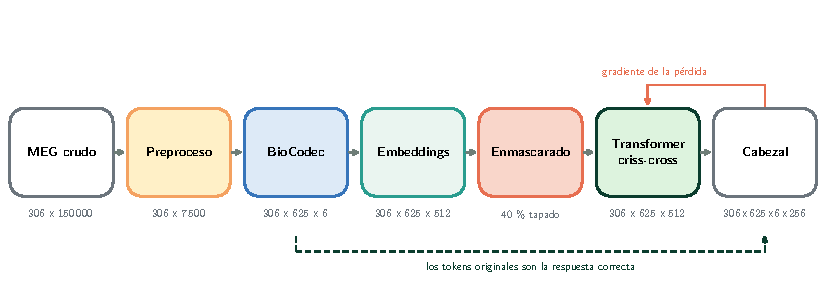
\includegraphics[width=\linewidth]{fig_pipeline.pdf}\par
  \vspace{3mm}
  \footnotesize
  Vamos a recorrer cada caja con las formas exactas de los tensores en cada punto. Fíjate ya en el doble papel del tokenizador: comprime la entrada \emph{y} fabrica la respuesta correcta que el cabezal tendrá que predecir.
  \note{Volveré a esta diapositiva entre bloque y bloque para situar dónde estamos.}
\end{frame}

% --- 21 ---
\begin{frame}[c]{Paso 0 --- Preprocesado (el terreno conocido)}
  \footnotesize
  \begin{columns}[t,totalwidth=\linewidth]
    \begin{column}{0.5\linewidth}
      \textbf{Filtrado y remuestreo}
      \begin{itemize}
        \item Paso alto a \term{0{,}1\,Hz}: elimina deriva lenta y artefactos del equipo.
        \item Paso bajo a \term{40\,Hz}.
        \item Remuestreo a \term{50\,Hz}.
      \end{itemize}
      \vspace{2mm}
      \textbf{Estandarización, por subsegmentos de 3\,s}
      \begin{enumerate}
        \item Corrección de línea base: restar la media por canal de los primeros \term{0{,}5\,s} del subsegmento.
        \item Escalar para que la mediana sea 0 y los cuartiles sean $-1$ y $+1$ (robusto frente a artefactos, a diferencia de $z$-score).
        \item Recortar (\eng{clamp}) al rango $[-5,5]$.
      \end{enumerate}
    \end{column}
    \begin{column}{0.48\linewidth}
      \begin{alertblock}{¿0{,}1\,Hz no mata el contexto largo?}
        No, el filtro elimina \term{componentes de frecuencia} por debajo de 0{,}1\,Hz. No elimina las \term{dependencias estadísticas} entre respuestas separadas por minutos. Son dos cosas distintas: contenido espectral $\neq$ escala temporal de las dependencias.
      \end{alertblock}
      \vspace{2mm}
      \begin{block}{¿Por qué estandarizar por subsegmentos de 3\,s?}
        Porque en la fase de ajuste la entrada estará formada por ventanas de 3\,s alineadas a palabras. Estandarizar igual en ambas fases hace que \term{el modelo vea la misma distribución} cuando se preentrena y cuando se ajusta.
      \end{block}
    \end{column}
  \end{columns}
\end{frame}

% --- 22 ---
\begin{frame}[c]{Paso 0 (bis) --- El elefante en la habitación: Nyquist}
  \small
  \begin{alertblock}{El problema}
    Paso bajo a 40\,Hz y remuestreo a 50\,Hz. Nyquist exige $f_s \geq 2 f_{\text{corte}} = 80$\,Hz. \term{Se está incumpliendo}, con riesgo de \eng{aliasing}.
  \end{alertblock}
  \vspace{1mm}
  \textbf{Por qué lo hacen igualmente:} para poder comparar exactamente con d'Ascoli et al.\ (2025), que usan ese mismo preprocesado, y porque bajar a 50\,Hz reduce a la mitad el número de instantes, que es lo que permite llegar a 150\,s de contexto.
  \vspace{2mm}
  \textbf{Y lo comprueban} (Apéndice C): repiten todo a 100\,Hz, que sí cumple Nyquist. Como eso duplica los instantes, hay que bajar el contexto de 150\,s a 75\,s por memoria de GPU.
  \vspace{1mm}
  \begin{center}
  \footnotesize
  \begin{tabular}{lcccccc}
    \toprule
    & \multicolumn{3}{c}{13\,\% de los datos} & \multicolumn{3}{c}{100\,\% de los datos} \\
    \cmidrule(lr){2-4}\cmidrule(lr){5-7}
    Modelo & MEG-MASC & Armeni & LibriBrain & MEG-MASC & Armeni & LibriBrain \\
    \midrule
    MEG-XL (50\,Hz, 150\,s)  & \textbf{47,0} & \textbf{54,9} & \textbf{57,3} & \textbf{46,4} & \textbf{61,2} & \textbf{63,0} \\
    MEG-XL (100\,Hz, 75\,s)  & 41,9 & 51,7 & 52,2 & 41,8 & 56,7 & 58,6 \\
    \bottomrule
  \end{tabular}
  \end{center}
  \vspace{1mm}
  \centering\small
  \term{Lectura:} el contexto largo compensa el \eng{aliasing}. Pero es una compensación empírica, no una justificación teórica.
  \note{Aquí es donde un neuroingeniero levantará la mano. Adelantarse y reconocer que el argumento es empírico.}
\end{frame}

% --- 23 ---
\begin{frame}[c]{Paso 1 --- Cuantización vectorial: un diccionario de formas de onda}
  \footnotesize
  \begin{columns}[T,totalwidth=\linewidth]
    \begin{column}{0.51\linewidth}
      \begin{block}{Cuantización vectorial (VQ)}
        \begin{enumerate}
          \item Tienes un \term{diccionario} (\eng{codebook}) de $V$ vectores prototipo, aprendidos previamente.
          \item Llega un vector de entrada.
          \item Buscas el prototipo \term{más parecido}.
          \item Transmites sólo \term{su índice}.
        \end{enumerate}
      \end{block}
      \vspace{1mm}
      {\scriptsize Es la idea de los cuantificadores vectoriales de los códecs de voz clásicos. Aquí $V = 256$ prototipos: 8 bits por símbolo.\par}
    \end{column}
    \begin{column}{0.46\linewidth}
      \centering
      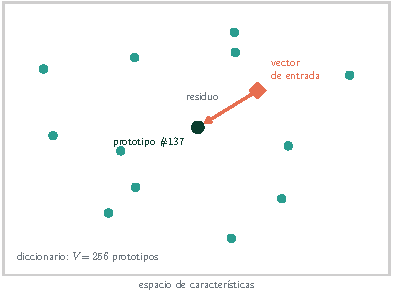
\includegraphics[width=\linewidth]{fig_vq.pdf}
    \end{column}
  \end{columns}
  \vspace{2mm}
  \centering\scriptsize
  \term{Pérdida inevitable:} sustituyes el vector real por el prototipo más cercano. Ese \term{residuo} es justo lo que motiva el siguiente paso.
\end{frame}

% --- 24 ---
\begin{frame}[c]{Paso 1 --- RVQ: cuantizar el error, seis veces}
  \centering
  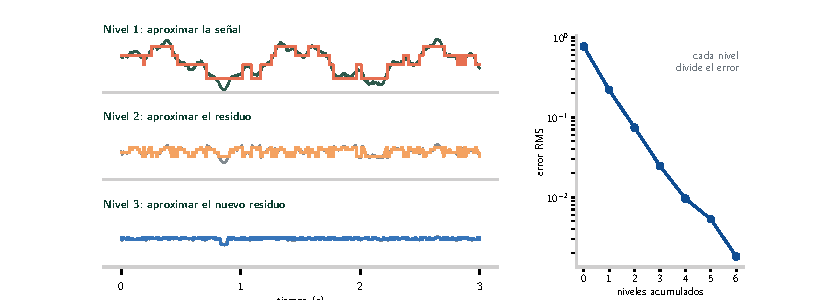
\includegraphics[width=\linewidth]{fig_rvq.pdf}\par
  \vspace{2mm}
  \begin{columns}[T,totalwidth=\linewidth]
    \begin{column}{0.52\linewidth}
      \scriptsize
      \term{Aproximación sucesiva}, como en un ADC: cada nivel cuantiza \emph{el residuo} del anterior. Con $Q = 6$ niveles de $V = 256$ prototipos se cubren $256^6 \approx 2{,}8\times10^{14}$ combinaciones guardando sólo $6\times256$ vectores.
    \end{column}
    \begin{column}{0.44\linewidth}
      \scriptsize
      La curva de la derecha está calculada de verdad: el error RMS cae de forma casi geométrica con cada nivel. Por eso los tokens residuales capturan bien la alta frecuencia.
    \end{column}
  \end{columns}
  \note{Analogía directa con un ADC de aproximaciones sucesivas o con codificación por capas.}
\end{frame}

% --- 25 ---
\begin{frame}[c]{Paso 1 --- BioCodec aplicado al MEG: las cifras exactas}
  \centering
  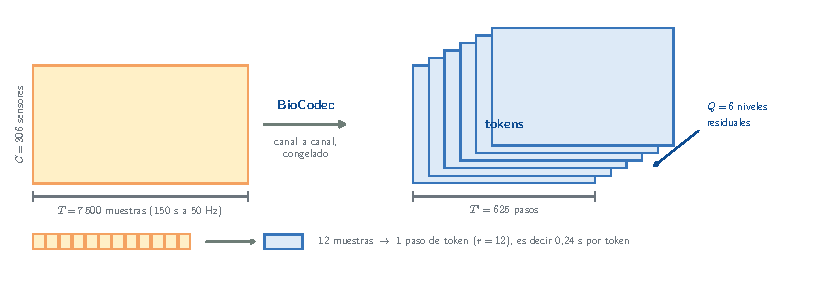
\includegraphics[width=\linewidth]{fig_tokenizer_shapes.pdf}\par
  \vspace{0.5mm}
  \begin{columns}[T,totalwidth=\linewidth]
    \begin{column}{0.44\linewidth}
      \scriptsize
      BioCodec (Avramidis et al., 2025) se entrenó con miles de horas de \term{EEG a 250\,Hz}. Se aplica \term{canal a canal}, sin mezclar sensores, y está \term{congelado}.
    \end{column}
    \begin{column}{0.53\linewidth}
      \scriptsize
      \setlength{\tabcolsep}{2pt}
      \renewcommand{\arraystretch}{1.0}
      \begin{tabular}{@{}ll@{\hspace{4mm}}ll@{}}
        \toprule
        Sensores & $C = 306$ & Posiciones & $306{\times}625 = 191\,250$ \\
        Muestras & $T = 7\,500$ & Tokens & $191\,250{\times}6 \approx 1{,}15$\,M \\
        Tras comprimir & $T' = 625$ & Resolución & $12/50 = 0{,}24$\,s \\
        \bottomrule
      \end{tabular}
    \end{column}
  \end{columns}
  \vspace{0.5mm}
  \centering\scriptsize
  \term{Doble función:} comprime la entrada $12\times$ \emph{y} fabrica las etiquetas del entrenamiento autosupervisado.
\end{frame}

% --- 26 ---
\begin{frame}[c]{Paso 1 --- Dos decisiones que merecen discusión}
  \small
  \begin{columns}[t,totalwidth=\linewidth]
    \begin{column}{0.48\linewidth}
      \begin{alertblock}{Un tokenizador de EEG, sobre MEG}
        BioCodec se entrenó con EEG a 250\,Hz. Aquí se usa sobre MEG a 50\,Hz. \term{Funciona}: lo eligen frente a BrainTokenizer (entrenado con MEG) porque reconstruye mejor.
        \vspace{1mm}
        \footnotesize Error de reconstrucción: \textbf{0{,}41} (BioCodec) frente a 0{,}69 (BrainTokenizer).
      \end{alertblock}
      {\footnotesize Es también la razón por la que el salto a EEG del TFM es razonable: parte del sistema \emph{ya viene} de EEG.}
    \end{column}
    \begin{column}{0.48\linewidth}
      \begin{block}{No comprimir el eje de sensores}
        BrainTokenizer comprime también entre canales; BioCodec no. Eso produce \term{más tokens} (peor para la memoria), pero \term{pierde menos información}.
        \vspace{1mm}
        Razonamiento explícito de los autores: \term{aún no sabemos qué partes de la señal son relevantes} para decodificar habla, así que conviene no descartar nada en el tokenizador y dejar que el transformer aprenda las relaciones entre canales.
      \end{block}
    \end{column}
  \end{columns}
  \vspace{2mm}
  \centering\small
  Consecuencia arquitectónica directa: como el eje de sensores \term{no} está comprimido, hay 306 posiciones espaciales por instante. Eso es justo lo que hace inviable la atención completa.
\end{frame}

% --- 27 ---
\begin{frame}[c]{Paso 2 --- De índices a vectores}
  \centering
  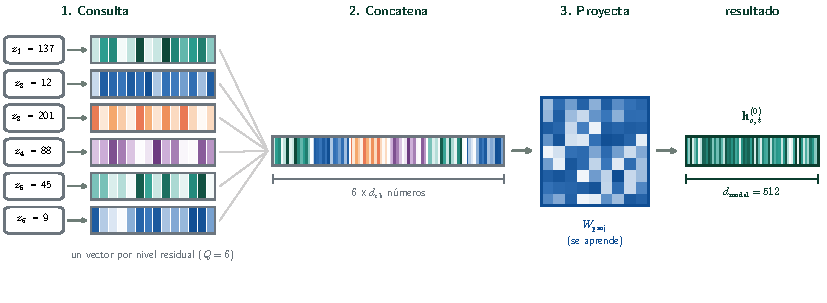
\includegraphics[width=\linewidth]{fig_indices_to_vectors.pdf}\par
  \vspace{1.2mm}
  {\footnotesize$\displaystyle \mathbf{h}^{(0)}_{c,t} = W_{\text{proj}}\big[\,\mathbf{e}^{(1)}_{z_{c,1,t}};\;\ldots\;;\;\mathbf{e}^{(Q)}_{z_{c,Q,t}}\,\big]$\par}
  \vspace{1.8mm}
  {\scriptsize Un índice (``prototipo \#137'') no puede entrar tal cual en una red: no hay relación numérica sensata entre el 137 y el 138. Los diccionarios $\mathbf{e}^{(q)}$ están \term{congelados} (vienen de BioCodec); $W_{\text{proj}}$ \term{sí se aprende}.\par}
  \note{Cada franja de color es un vector. Señalar que la concatenación conserva los seis colores: se ve que son seis trozos pegados.}
\end{frame}

% --- 28 ---
\begin{frame}[c]{Paso 2 --- El modelo no sabe dónde está cada sensor}
  \small
  \begin{alertblock}{El problema}
    Hasta ahora, $\mathbf{h}^{(0)}_{c,t}$ sólo describe \term{la forma de onda}. El modelo no tiene ni idea de si el canal $c$ está sobre el lóbulo temporal izquierdo o sobre el occipital. Y distintos equipos MEG tienen distinto número y disposición de sensores.
  \end{alertblock}
  \vspace{2mm}
  \textbf{Solución: describir cada sensor por lo que físicamente es.} Tres piezas de información que ya están en el fichero de la grabación:
  \begin{columns}[t,totalwidth=\linewidth]
    \begin{column}{0.32\linewidth}
      \begin{block}{Posición $\mathbf{p}_c \in \mathbb{R}^3$}
        \scriptsize Coordenadas 3D de la bobina en el casco.
      \end{block}
    \end{column}
    \begin{column}{0.32\linewidth}
      \begin{block}{Orientación $\mathbf{o}_c \in \mathbb{R}^3$}
        \scriptsize Hacia dónde apunta. Determina qué componente del campo mide.
      \end{block}
    \end{column}
    \begin{column}{0.32\linewidth}
      \begin{block}{Tipo de sensor}
        \scriptsize Magnetómetro o gradiómetro. Categoría discreta.
      \end{block}
    \end{column}
  \end{columns}
  \vspace{2mm}
  \centering\small
  Ventaja clave: así el modelo puede entrenarse con \term{varios sistemas MEG distintos sin cambiar la arquitectura}. No aprende ``el canal 42'', aprende ``un sensor situado aquí, orientado así''.
  \note{Este es el punto que más se transfiere al TFM: la representación de sensores es lo que permite reutilizar el modelo en EEG.}
\end{frame}

% --- 29 ---
\begin{frame}[c]{Paso 2 --- Por qué las coordenadas no se meten tal cual}
  \footnotesize
  Meter $(x,y,z)$ tal cual funciona mal: las redes densas tienden a funciones \term{suaves} y no separan sensores cercanos. La solución: \term{características de Fourier gaussianas}, $\gamma(\mathbf{v}) = [\cos(2\pi B\mathbf{v}),\ \sin(2\pi B\mathbf{v})]$, con $B$ de frecuencias espaciales sorteadas de $\mathcal{N}(0,\sigma^2)$ y \term{fijas} después.
  \vspace{1mm}
  \centering
  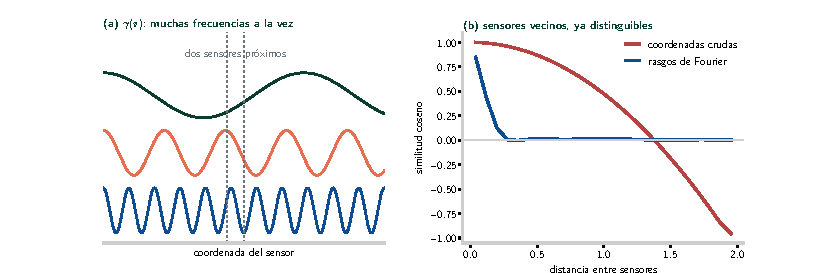
\includegraphics[width=\linewidth]{fig_fourier.pdf}\par
  \vspace{1mm}
  {\scriptsize El panel (b) está calculado sobre 400 sensores en un casco esférico: con coordenadas crudas dos vecinos son casi indistinguibles; sus rasgos de Fourier se separan enseguida. \quad $d_{\text{fourier}} = 256$;\; $\sigma_{\text{pos}} = 1{,}8$;\; $\sigma_{\text{orient}} = 1{,}0$.\par}
\end{frame}

% --- 30 ---
\begin{frame}[c]{Paso 2 --- La suma final}
  \centering
  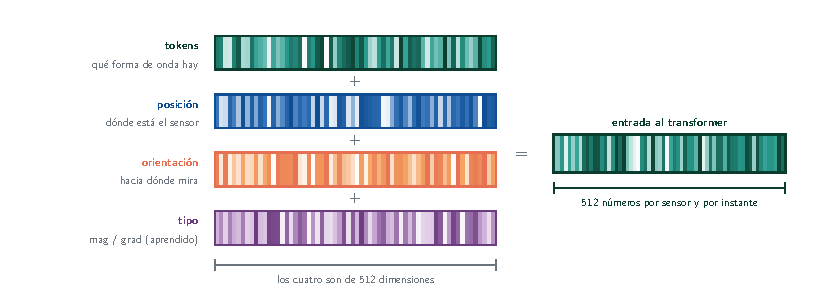
\includegraphics[width=\linewidth]{fig_sum_embeddings.pdf}\par
  \vspace{2.5mm}
  \begin{columns}[T,totalwidth=\linewidth]
    \begin{column}{0.48\linewidth}
      \scriptsize Se \term{suman}, no se concatenan: así la dimensión no crece y cada aportación se superpone sobre la misma representación.
    \end{column}
    \begin{column}{0.48\linewidth}
      \scriptsize Resultado: un tensor $H^{(0)}$ de tamaño $306 \times 625 \times 512$. Unos \term{98 millones de números} por muestra de 2,5 minutos.
    \end{column}
  \end{columns}
\end{frame}

% --- 31 ---
\begin{frame}[c]{Paso 3 --- La idea de la atención \emph{criss-cross}}
  \footnotesize
  Atención completa sobre $306 \times 625 = 191\,250$ posiciones es imposible. La solución: \term{no mirar todos los pares}, sólo los que comparten fila o columna.
  \vspace{0.5mm}
  \centering
  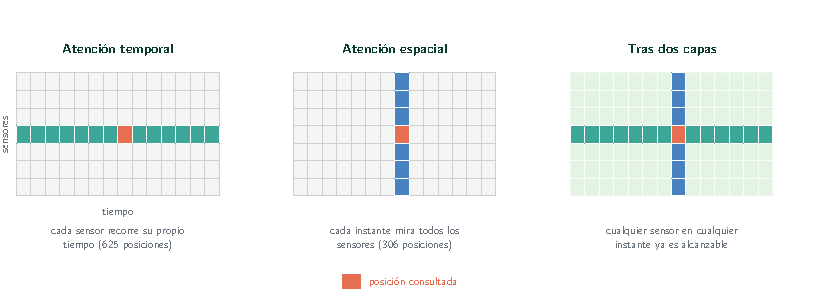
\includegraphics[width=\linewidth]{fig_crisscross.pdf}\par
  \vspace{1mm}
  {\scriptsize Con dos capas seguidas, cualquier sensor en cualquier instante puede alcanzar a cualquier otro: primero por la fila, luego por la columna. De esa cruz viene el nombre.\par}
  \note{Analogía: en vez de conectar todas las casas con todas, se conecta cada calle y cada avenida. Con dos saltos se llega a cualquier sitio.}
\end{frame}

% --- 32 ---
\begin{frame}[c]{Paso 3 --- Cómo se combinan las dos atenciones}
  \small
  MEG-XL no las aplica en serie, sino \term{en paralelo, partiendo el vector de características por la mitad}:
  \[
    H^{(\ell)} = H^{(\ell-1)} + \Big[\ \underbrace{\text{AtenciónEspacial}\big(H^{(\ell-1)}_{:d/2}\big)}_{\text{primeras 256 componentes}}\ ;\ \underbrace{\text{AtenciónTemporal}\big(H^{(\ell-1)}_{d/2:}\big)}_{\text{últimas 256 componentes}}\ \Big]
  \]
  \vspace{1mm}
  \begin{columns}[t,totalwidth=\linewidth]
    \begin{column}{0.5\linewidth}
      \textbf{Lectura de la fórmula, término a término}
      \begin{itemize}\footnotesize
        \item Las 512 componentes se cortan en dos mitades de 256.
        \item La primera mitad se procesa \term{sólo} con atención entre sensores.
        \item La segunda mitad, \term{sólo} con atención a lo largo del tiempo.
        \item Se vuelven a pegar (concatenación) y se \term{suman a la entrada}: es la conexión residual.
      \end{itemize}
    \end{column}
    \begin{column}{0.48\linewidth}
      \textbf{Consecuencias prácticas}
      \begin{itemize}\footnotesize
        \item Las dos atenciones se calculan \term{a la vez}: mitad del coste de hacerlas en serie.
        \item Son independientes dentro de una capa; la mezcla entre ambas mitades la hace la \term{red densa} del bloque, que sí ve las 512 componentes.
        \item RoPE se aplica sólo en la rama temporal.
      \end{itemize}
    \end{column}
  \end{columns}
\end{frame}

% --- 33 ---
\begin{frame}[c]{Paso 3 --- El ahorro, con los números encima de la mesa}
  \centering
  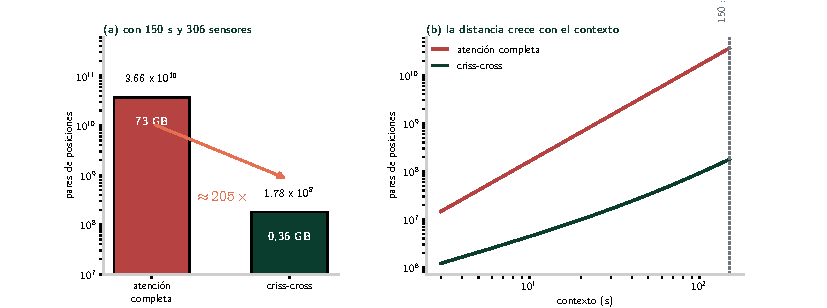
\includegraphics[width=\linewidth]{fig_cost.pdf}\par
  \vspace{1.5mm}
  \begin{columns}[T,totalwidth=\linewidth]
    \begin{column}{0.48\linewidth}
      \scriptsize
      \vspace{-2mm}
      \[ \mathcal{O}\big((C\,T')^2\big) \;\longrightarrow\; \mathcal{O}\big(C\,T'^2 + T'\,C^2\big) \]
      \vspace{-4mm}
      \par Los 73\,GB son sólo la matriz de pesos, y además \term{por capa y por cabeza}.
    \end{column}
    \begin{column}{0.48\linewidth}
      \scriptsize
      \term{Lo que se pierde:} dentro de una sola capa, la posición (sensor 12, instante 300) no puede mirar directamente a (sensor 200, instante 10). Necesita dos saltos; con 8 capas hay de sobra.
    \end{column}
  \end{columns}
\end{frame}

% --- 34 ---
\begin{frame}[c]{Paso 3 --- Ficha técnica de la red}
  \small
  \begin{columns}[t,totalwidth=\linewidth]
    \begin{column}{0.5\linewidth}
      \begin{block}{Arquitectura}
        \footnotesize
        \begin{tabular}{@{}ll@{}}
          \toprule
          Capas $L$ & 8 \\
          Dimensión $d_{\text{model}}$ & 512 \\
          Cabezas de atención & 8 \\
          Normalización & RMSNorm, pre-LN \\
          Atención & \emph{criss-cross} \\
          Red densa & expansión $4\times$, SELU \\
          Posición temporal & RoPE \\
          \textbf{Parámetros} & \textbf{$\approx$20\,M} \\
          \bottomrule
        \end{tabular}
      \end{block}
    \end{column}
    \begin{column}{0.48\linewidth}
      \begin{block}{Detalle que resuelve un problema real}
        Distintos sistemas MEG tienen distinto número de sensores. MEG-XL \term{rellena} hasta un número máximo de canales y usa una \term{máscara de sensores} que excluye los canales de relleno:
        \begin{itemize}\footnotesize
          \item del cálculo de la atención, y
          \item del cálculo de la pérdida.
        \end{itemize}
        \vspace{1mm}
        Gracias a eso se puede entrenar con CamCAN, MOUS y SMN4Lang \term{mezclados}, sin tocar la arquitectura.
      \end{block}
      {\footnotesize\color{muted} Esta misma máscara es la pieza que el TFM reutiliza para montajes EEG heterogéneos.}
    \end{column}
  \end{columns}
\end{frame}

% --- 35 ---
\begin{frame}[c]{Paso 4 --- El enmascaramiento, con todos sus porqués}
  \centering
  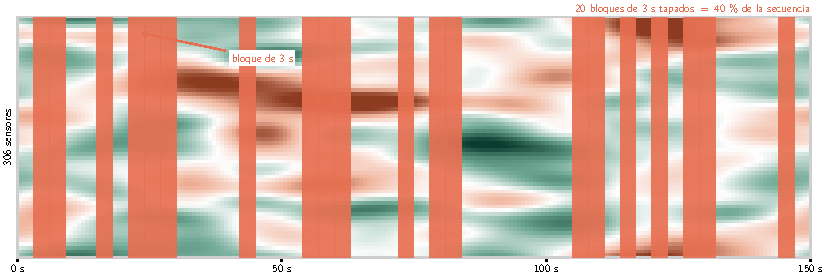
\includegraphics[width=\linewidth]{fig_masking.pdf}\par
  \vspace{1.5mm}
  \begin{columns}[T,totalwidth=\linewidth]
    \begin{column}{0.49\linewidth}
      \scriptsize
      \term{¿Por qué bloques de 3\,s y no muestras sueltas?} El MEG está fuertemente autocorrelado: tapar una muestra aislada se resuelve interpolando entre vecinas. Además, 3\,s es la duración típica de la respuesta neural decodificable a una palabra.
    \end{column}
    \begin{column}{0.49\linewidth}
      \scriptsize
      \term{¿Por qué la misma máscara en todos los sensores?} Si se tapara un sensor y no sus vecinos, el modelo copiaría del de al lado en el mismo instante. Tapando la columna entera, la única salida es usar el \term{contexto temporal}.
    \end{column}
  \end{columns}
  \vspace{1mm}
  \centering\scriptsize
  Los tokens tapados se sustituyen por un \term{vector de máscara aprendido}, y la pérdida se calcula sólo sobre esas posiciones.
  \note{El diseño de la máscara es lo que fuerza a aprender contexto largo. Es el corazón conceptual del método.}
\end{frame}

% --- 36 ---
\begin{frame}[c]{Paso 4 --- ¿Por qué justo el 40\,\%?}
  \footnotesize
  Es un hiperparámetro ajustado a mano, pero el artículo lo sitúa en su contexto, y es informativo:
  \vspace{1mm}
  \centering
  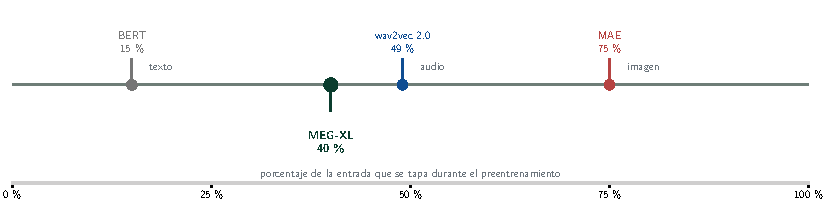
\includegraphics[width=\linewidth]{fig_mask_ratio.pdf}\par
  \vspace{1.5mm}
  \begin{itemize}\scriptsize
    \item \term{Texto (15\,\%)}: cada palabra lleva mucha información. Tapar mucho hace la tarea imposible.
    \item \term{Imagen (75\,\%)}: los píxeles vecinos son casi idénticos. Hay que tapar muchísimo para que la tarea no sea trivial.
    \item \term{Audio y MEG ($\sim$40--50\,\%)}: señales muy redundantes en el tiempo, pero no tanto como una imagen. MEG-XL cae donde cabía esperar, junto a un modelo de habla.
  \end{itemize}
\end{frame}

% --- 37 ---
\begin{frame}[c]{Paso 5 --- Predicción y pérdida}
  \footnotesize
  Para cada posición tapada $(c,t)$, se toma la salida de la última capa $\mathbf{h}^{(L)}_{c,t}$ (512 números) y se predicen \term{los 6 índices} de golpe, con 6 clasificadores lineales independientes:
  \[ p\big(z_{c,q,t}\mid X_{\setminus M}\big) = \mathrm{softmax}\big(W_q\,\mathbf{h}^{(L)}_{c,t}\big), \qquad q = 1,\ldots,6 \]
  \vspace{-2mm}
  \begin{columns}[t,totalwidth=\linewidth]
    \begin{column}{0.54\linewidth}
      Cada $W_q$ produce \term{256 números}, uno por prototipo del diccionario $q$; la \eng{softmax} los convierte en probabilidades que suman 1.
      \vspace{2mm}
      La pérdida es la \term{entropía cruzada} promediada sobre todas las posiciones tapadas, todos los sensores y los 6 niveles:
      \[ \mathcal{L} = -\frac{1}{|M|\,C\,Q}\sum_{t\in M}\sum_{c=1}^{C}\sum_{q=1}^{Q}\log p\big(z_{c,t,q}\mid X_{\setminus M}\big) \]
    \end{column}
    \begin{column}{0.44\linewidth}
      \begin{block}{Qué significa esa fórmula}
        \footnotesize
        ``Mira la probabilidad que el modelo asignó al índice \term{correcto}; si es alta, el logaritmo es casi 0 y no penaliza; si es baja, el $-\log$ se dispara.''
        \vspace{1.5mm}
        El nivel de azar es $1/256 \approx 0{,}4\,\%$.
      \end{block}
      \vspace{1mm}
      \begin{exampleblock}{Interpretación}
        Es el mismo tipo de pérdida que usarías para clasificar época por época en un clasificador de estadios de sueño. Aquí sólo hay muchísimas más clasificaciones simultáneas.
      \end{exampleblock}
    \end{column}
  \end{columns}
\end{frame}

% --- 38 ---
\begin{frame}[c]{Resumen: las formas del tensor en cada paso}
  \centering
  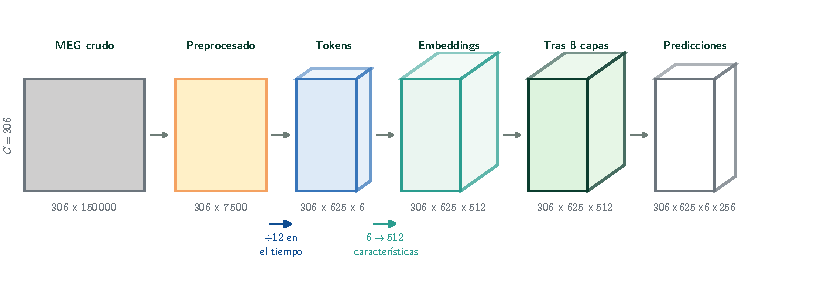
\includegraphics[width=\linewidth]{fig_tensor_shapes.pdf}\par
  \vspace{2mm}
  \begin{columns}[c,totalwidth=\linewidth]
    \begin{column}{0.33\linewidth}\centering\smallmetric{0,24\,s}{cubre cada paso de token}\end{column}
    \begin{column}{0.33\linewidth}\centering\smallmetric{191\,250}{posiciones de entrada}\end{column}
    \begin{column}{0.33\linewidth}\centering\smallmetric{40\,\%}{de la secuencia tapado}\end{column}
  \end{columns}
  \vspace{2mm}
  \centering\scriptsize
  Los dos únicos cambios de escala reales: el tokenizador divide el tiempo entre 12, y el embedding pasa de 6 índices a 512 características.
  \note{Diapositiva de referencia. Si alguien se ha perdido, aquí se recupera.}
\end{frame}

% --- 39 ---
\begin{frame}[c]{Hiperparámetros del preentrenamiento}
  \small
  \begin{columns}[t,totalwidth=\linewidth]
    \begin{column}{0.48\linewidth}
      \begin{block}{Datos}
        \footnotesize
        \begin{tabular}{@{}ll@{}}
          \toprule
          Frecuencia original & 1000\,Hz \\
          Remuestreo & 50\,Hz \\
          Paso bajo / paso alto & 40\,Hz / 0,1\,Hz \\
          Estandarización & IQR $=[-1,1]$ por 3\,s \\
          Línea base & $[0{,}0;\,0{,}5]$\,s por 3\,s \\
          Recorte & $[-5,5]$ \\
          Longitud de muestra & 150\,s \\
          \bottomrule
        \end{tabular}
      \end{block}
      \begin{block}{Corpus de preentrenamiento}
        \footnotesize
        \begin{tabular}{@{}lll@{}}
          \toprule
          CamCAN & $\sim$700 suj. & reposo, sensorimotor \\
          MOUS & 104 suj. & escucha (neerlandés) \\
          SMN4Lang & 12 suj. & escucha (mandarín) \\
          \midrule
          \multicolumn{3}{l}{\textbf{$\approx$300 horas, $>$800 sujetos}} \\
          \bottomrule
        \end{tabular}
      \end{block}
    \end{column}
    \begin{column}{0.48\linewidth}
      \begin{block}{Optimización}
        \footnotesize
        \begin{tabular}{@{}ll@{}}
          \toprule
          Pasos de entrenamiento & 35\,000 \\
          Tamaño de lote & 1 \\
          Tasa de aprendizaje & $10^{-4}$ \\
          Decaimiento de pesos & $10^{-4}$ \\
          Calentamiento & 250 pasos \\
          Recorte de gradiente & 1,0 \\
          Optimizador & AdamW \\
          Pérdida & entropía cruzada \\
          \bottomrule
        \end{tabular}
      \end{block}
      \begin{alertblock}{Tamaño de lote $=$ 1}
        \footnotesize Una única muestra de 2,5 minutos ya ocupa toda la GPU. El ``lote'' efectivo son los $\approx$1,15\,M de tokens que contiene.
      \end{alertblock}
      {\footnotesize\color{muted} Preentrenamiento: $\approx$12\,h en una H100.}
    \end{column}
  \end{columns}
\end{frame}

% #############################################################################
\section{De la señal a la palabra: ajuste y resultados}
% #############################################################################

% --- 40 ---
\begin{frame}[c]{La tarea: decodificación contextual de palabras}
  \small
  Se sigue exactamente el protocolo de d'Ascoli et al.\ (2025), para que la comparación sea limpia.
  \vspace{2mm}
  \begin{center}
  \resizebox{0.95\textwidth}{!}{%
  \begin{tikzpicture}
    \draw[line width=.8pt, draw=linegray] (0,2.2) -- (12,2.2);
    \foreach \i/\w in {0/the, 1/fruit, 2/bowl, 3/had, 4/a, 5/pineapple}{
      \draw[draw=deepgreen!60, fill=softgreen, rounded corners=2pt] (\i*2.0+0.1,2.0) rectangle ++(1.8,0.4);
      \node[font=\scriptsize] at (\i*2.0+1.0,2.2) {\w};
      \draw[draw=accent, fill=accent!12, rounded corners=2pt] (\i*2.0+0.1,0.9) rectangle ++(1.8,0.75);
      \node[font=\tiny, text=accent!70!black, align=center] at (\i*2.0+1.0,1.27) {ventana 3\,s\\ \tiny desde $-0{,}5$\,s};
      \draw[ar, gray!70] (\i*2.0+1.0,1.95) -- (\i*2.0+1.0,1.7);
    }
    \node[font=\scriptsize, anchor=west] at (12.1,2.2) {estímulo};
    \draw[decorate, decoration={brace, amplitude=4pt, mirror}, draw=deepgreen] (0.1,0.6) -- (11.9,0.6);
    \node[font=\scriptsize, text=deepgreen, anchor=north, align=center] at (6,0.4) {$N = 50$ palabras $\times$ 3\,s $=$ 150\,s de entrada, concatenadas en el eje temporal};
  \end{tikzpicture}}
  \end{center}
  \vspace{2mm}
  \begin{columns}[t,totalwidth=\linewidth]
    \begin{column}{0.5\linewidth}
      \begin{itemize}\footnotesize
        \item Cada ventana empieza \term{0{,}5\,s antes} del inicio de la palabra y dura \term{3\,s}.
        \item Se concatenan 50 ventanas $\rightarrow$ \term{exactamente 150\,s}, la misma longitud del preentrenamiento. Por eso no hace falta tocar la arquitectura.
      \end{itemize}
    \end{column}
    \begin{column}{0.48\linewidth}
      \begin{alertblock}{Honestidad sobre el montaje}
        \footnotesize Esa entrada \term{no es continua en tiempo fisiológico}: se pegan trozos. Se hace así para replicar exactamente la línea base y para eliminar el efecto de la velocidad variable del habla.
      \end{alertblock}
    \end{column}
  \end{columns}
\end{frame}

% --- 41 ---
\begin{frame}[c]{¿Contra qué se compara la salida? Un embedding lingüístico}
  \footnotesize
  El modelo \term{no clasifica entre 50 palabras}. Predice un \term{vector que describe el significado} de la palabra, y luego se busca la palabra más parecida.
  \vspace{2mm}
  \begin{center}
  \resizebox{0.80\textwidth}{!}{%
  \begin{tikzpicture}[node distance=7mm]
    \node[blkg, minimum width=2.1cm, minimum height=1.2cm] (brain) {salida del\\transformer\\ \scriptsize $\mathbf{h}^{(L)}$};
    \node[blk, right=of brain, minimum width=2.2cm, minimum height=1.2cm] (pool) {promediar en\\el tiempo de\\la palabra\\ \scriptsize y aplanar canales};
    \node[blkr, right=of pool, minimum width=1.8cm, minimum height=1.2cm] (mlp) {MLP\\ \scriptsize oculta 2048};
    \node[blkb, right=of mlp, minimum width=2.0cm, minimum height=1.2cm] (pred) {$\hat{\mathbf{w}}_n$\\ \scriptsize vector predicho};
    \foreach \a/\b in {brain/pool, pool/mlp, mlp/pred}{\draw[ar] (\a)--(\b);}

    \node[blky, below=13mm of pred, minimum width=2.0cm, minimum height=1.2cm] (true) {$\mathbf{w}_n$\\ \scriptsize vector objetivo};
    \node[blk, left=of true, minimum width=2.6cm, minimum height=1.2cm] (t5) {modelo de lenguaje\\\textbf{T5}\\ \scriptsize convierte ``pineapple''\\ \scriptsize en un vector};
    \draw[ar] (t5) -- (true);
    \draw[{Latex[length=2.2mm]}-{Latex[length=2.2mm]}, accent, line width=1pt] (pred) -- node[right, font=\scriptsize, text=accent, align=left] {acercar\\(pérdida contrastiva)} (true);
  \end{tikzpicture}}
  \end{center}
  \vspace{2mm}
  \footnotesize
  \begin{itemize}
    \item \term{T5} es un modelo de lenguaje preentrenado; se usa sólo como \term{traductor de palabra a vector}, congelado. Palabras de significado parecido dan vectores parecidos.
    \item Ventaja sobre clasificar directamente: el modelo puede acertar ``parcialmente'' y, en principio, generalizar a palabras que no vio.
  \end{itemize}
\end{frame}

% --- 42 ---
\begin{frame}[c]{La pérdida contrastiva, sin jerga}
  \small
  \begin{columns}[c,totalwidth=\linewidth]
    \begin{column}{0.5\linewidth}
      Dentro de cada lote de 50 palabras, la pérdida (\term{SigLIP}, variante D-SigLIP) hace dos cosas a la vez:
      \begin{itemize}
        \item \term{Acercar} el vector predicho al vector de \emph{su} palabra.
        \item \term{Alejarlo} de los vectores de las otras 49 palabras del lote.
      \end{itemize}
      \vspace{2mm}
      {\footnotesize Detalle fino: la variante usada \term{enmascara las palabras repetidas} dentro del lote, para no penalizar por ``alejarse'' de un vector que en realidad es el correcto.}
      \vspace{2mm}
      \begin{block}{Por qué no basta con minimizar la distancia}
        \footnotesize Si sólo se acercara, el modelo podría colapsar y predecir siempre el mismo vector medio. El empuje hacia fuera es lo que obliga a \term{discriminar}.
      \end{block}
    \end{column}
    \begin{column}{0.47\linewidth}
      \centering
      \resizebox{0.92\linewidth}{!}{%
      \begin{tikzpicture}
        \draw[draw=gray!35] (0,0) circle (2.6cm);
        \filldraw[deepgreen] (0.55,0.75) circle (3pt) node[above right, font=\scriptsize] {``pineapple''};
        \filldraw[accent] (-0.15,0.05) circle (3pt) node[below left, font=\scriptsize, text=accent] {predicción};
        \draw[-{Latex[length=2mm]}, accent, line width=1pt] (-0.1,0.12) -- (0.42,0.63);
        \foreach \x/\y in {-1.7/1.2, 1.9/-0.8, -1.2/-1.7, 1.5/1.6, -2.1/-0.2}{
          \filldraw[muted!70] (\x,\y) circle (2.4pt);
          \draw[-{Latex[length=1.6mm]}, muted, line width=.5pt, dashed] (-0.1,0.05) -- ($(-0.1,0.05)!0.35!(\x,\y)$);
        }
        \node[font=\scriptsize, text=muted, anchor=west] at (1.4,-1.9) {otras palabras};
      \end{tikzpicture}}
    \end{column}
  \end{columns}
\end{frame}

% --- 43 ---
\begin{frame}[c]{Inferencia y métrica}
  \small
  \begin{columns}[t,totalwidth=\linewidth]
    \begin{column}{0.5\linewidth}
      \begin{block}{Cómo se decide la palabra}
        Se toma el vector predicho $\hat{\mathbf{w}}_n$ y se compara con el vector de cada palabra del \term{vocabulario de recuperación}:
        \[ \hat{y}_n = \arg\max_{y}\ \cos(\hat{\mathbf{w}}_n, \mathbf{w}_y) \]
        Es una búsqueda del \term{vecino más próximo} por similitud coseno. Nada más.
      \end{block}
      \vspace{1mm}
      {\footnotesize Vocabulario: las 50 palabras más frecuentes (y, en el apéndice, las 250 más frecuentes).}
    \end{column}
    \begin{column}{0.48\linewidth}
      \begin{alertblock}{Métrica: Top-10 balanceada}
        \begin{itemize}\footnotesize
          \item \term{Top-10}: se cuenta acierto si la palabra correcta está entre las 10 más parecidas.
          \item \term{Balanceada}: macro-media \term{por clase de palabra}, no media sobre ejemplos.
        \end{itemize}
        \vspace{1mm}
        \footnotesize \term{Por qué balanceada:} sin ello, acertar siempre ``the'' y ``a'' infla la cifra. El nivel de azar queda en $10/50 = 20\,\%$ (o $10/250 = 4\,\%$).
      \end{alertblock}
    \end{column}
  \end{columns}
  \vspace{2mm}
  \centering\small
  \term{Al leer cualquier número de las tablas siguientes, el azar es 20\,\%.} Un 47\,\% no es ``poco'': es más del doble del azar en una tarea con SNR pésima.
  \note{Muy importante para una audiencia que no está acostumbrada a estas métricas: recordar el azar antes de enseñar las tablas.}
\end{frame}

% --- 44 ---
\begin{frame}[c]{Hiperparámetros del ajuste fino}
  \small
  \begin{columns}[c,totalwidth=\linewidth]
    \begin{column}{0.48\linewidth}
      \begin{block}{Ajuste}
        \footnotesize
        \begin{tabular}{@{}ll@{}}
          \toprule
          Dimensión oculta del MLP & 2048 \\
          Épocas máximas & 50 \\
          Parada temprana (paciencia) & 10 épocas \\
          Criterio de parada & Top-10 bal.\ en validación \\
          Tamaño de lote & 50 palabras \\
          LR del transformer & $10^{-5}$ \\
          LR del MLP & $10^{-3}$ \\
          Decaimiento de pesos & $10^{-4}$ \\
          Optimizador & AdamW \\
          Pérdida & D-SigLIP \\
          \bottomrule
        \end{tabular}
      \end{block}
    \end{column}
    \begin{column}{0.48\linewidth}
      \begin{exampleblock}{Un detalle revelador}
        El transformer se ajusta con una tasa \term{100 veces menor} que el MLP.
        \vspace{1.5mm}
        Razón: el transformer ya \term{sabe algo} y sólo hay que retocarlo con cuidado para no borrar lo aprendido; el MLP empieza de cero y necesita moverse rápido.
      \end{exampleblock}
      \vspace{1mm}
      \begin{block}{Datos de evaluación}
        \footnotesize
        \begin{tabular}{@{}lccc@{}}
          \toprule
          Conjunto & Suj. & h/suj. & h total \\
          \midrule
          MEG-MASC & 27 & 2 & 54 \\
          Armeni & 3 & 10 & 30 \\
          LibriBrain & 1 & 52 & 52 \\
          \bottomrule
        \end{tabular}
        \vspace{1mm}
        \\ Particiones 80:10:10, con \term{el mismo estímulo siempre en la misma partición}.
      \end{block}
    \end{column}
  \end{columns}
\end{frame}

% --- 45 ---
\begin{frame}[c]{Resultado 1 --- Contra otros modelos fundacionales}
  \centering
  \scriptsize
  \renewcommand{\arraystretch}{1.15}
  \setlength{\tabcolsep}{5pt}
  \begin{tabular}{lccccccc}
    \toprule
    & & \multicolumn{3}{c}{\textbf{Con el 13\,\% de los datos}} & \multicolumn{3}{c}{\textbf{Con el 100\,\% de los datos}} \\
    \cmidrule(lr){3-5}\cmidrule(lr){6-8}
    Modelo & Par. & MEG-MASC & Armeni & LibriBrain & MEG-MASC & Armeni & LibriBrain \\
    \midrule
    BioCodec   & 1,0\,M & 19,8 & 20,0 & 19,9 & 31,2 & 37,1 & 41,9 \\
    EEGPT      & 4,7\,M & 19,6 & 20,3 & 20,3 & 26,3 & 20,8 & 22,9 \\
    BIOT       & 3,2\,M & 20,0 & 20,2 & 20,6 & 31,3 & 35,7 & 45,6 \\
    BBL        & 15\,M  & 21,5 & 22,3 & 32,1 & 35,9 & 39,1 & 49,9 \\
    BrainOmni  & 8,4\,M & 18,7 & 21,0 & 29,7 & 19,1 & \textbf{62,3} & 63,0 \\
    LaBraM     & 5,8\,M & 33,2 & 26,3 & 40,3 & 31,1 & 42,0 & 47,7 \\
    \midrule
    \textbf{MEG-XL} & \textbf{20\,M} & \textbf{47,0} & \textbf{54,9} & \textbf{57,3} & \textbf{46,4} & 61,2 & \textbf{63,0} \\
    \midrule
    \emph{Azar} & --- & \emph{20,0} & \emph{20,0} & \emph{20,0} & \emph{20,0} & \emph{20,0} & \emph{20,0} \\
    \bottomrule
  \end{tabular}
  \vspace{2mm}
  \begin{columns}[t,totalwidth=\linewidth]
    \begin{column}{0.48\linewidth}
      \begin{alertblock}{Lo importante está en la mitad izquierda}
        \footnotesize Con pocos datos, \term{casi todos los demás modelos se quedan en el azar} (19--21\,\%). MEG-XL llega a 47--57\,\%. Ese es el régimen clínicamente relevante.
      \end{alertblock}
    \end{column}
    \begin{column}{0.48\linewidth}
      \begin{block}{Y un matiz honesto}
        \footnotesize BrainOmni gana en Armeni con todos los datos (62,3 frente a 61,2) pero se hunde en MEG-MASC (19,1). Es decir: funciona con pocos sujetos y muchas horas, no al revés.
      \end{block}
    \end{column}
  \end{columns}
\end{frame}

% --- 46 ---
\begin{frame}[c]{Resultado 2 --- Eficiencia de datos frente al supervisado}
  \footnotesize
  \begin{columns}[c,totalwidth=\linewidth]
    \begin{column}{0.46\linewidth}
      \begin{itemize}
        \item \term{MEG-MASC} (27 sujetos, 2\,h cada uno): MEG-XL mejora al supervisado hasta en un 25\,\% y la ventaja \term{se mantiene con todos los datos}.
        \item \term{Armeni} (3 sujetos, 10\,h): unos 10 puntos por encima hasta las $\sim$15\,h.
        \item \term{LibriBrain} (1 sujeto, 52\,h): empatan hasta las 2,5\,h; a partir de ahí \term{gana el supervisado}.
      \end{itemize}
      \vspace{2mm}
      \begin{exampleblock}{La regla que emerge}
        \footnotesize El preentrenamiento sustituye datos \term{del sujeto}, no datos en general. Muchos sujetos poco tiempo $\rightarrow$ gana preentrenar. Un sujeto muchísimo tiempo $\rightarrow$ gana entrenar desde cero.
      \end{exampleblock}
    \end{column}
    \begin{column}{0.5\linewidth}
      \centering
      \resizebox{\linewidth}{!}{%
      \begin{tikzpicture}
        \draw[ar] (0,0) -- (7.2,0) node[right, font=\scriptsize] {horas de ajuste (log)};
        \draw[ar] (0,0) -- (0,4.2) node[above, font=\scriptsize] {Top-10};
        \draw[dashed, gray!60] (0,0.8) -- (7,0.8) node[right, font=\tiny, text=muted] {azar};
        \draw[draw=deepgreen, line width=1.2pt] (0.3,2.0) .. controls (2,3.0) and (4,3.3) .. (6.8,3.5);
        \node[font=\scriptsize, text=deepgreen, anchor=west] at (0.5,2.35) {MEG-XL preentrenado};
        \draw[draw=accent, line width=1.2pt] (0.3,0.85) .. controls (2.2,1.1) and (4.2,2.6) .. (6.8,3.75);
        \node[font=\scriptsize, text=accent, anchor=west] at (4.4,2.35) {supervisado};
        \draw[draw=muted, line width=1pt, dash pattern=on 3pt off 2pt] (0.3,0.82) .. controls (2.5,1.0) and (4.5,1.9) .. (6.8,2.5);
        \node[font=\scriptsize, text=muted, anchor=west] at (3.0,1.35) {MEG-XL sin preentrenar};
        \draw[dotted, gray, line width=.8pt] (5.4,0) -- (5.4,4.0);
        \node[font=\tiny, text=muted, anchor=south, align=center] at (5.4,4.0) {cruce};
      \end{tikzpicture}}
      \vspace{1mm}
      {\tiny\color{muted}Esquema cualitativo de la Figura 3.}
    \end{column}
  \end{columns}
  \vspace{1mm}
  \centering\footnotesize
  \term{El control más importante:} MEG-XL \emph{sin} preentrenar va muy por debajo. La ganancia viene del preentrenamiento, no de la arquitectura.
\end{frame}

% --- 47 ---
\begin{frame}[c]{Resultado 3 --- Más contexto, mejores representaciones}
  \small
  \textbf{Experimento:} preentrenar varios modelos con contextos de 15, 30, 45\ldots 150\,s; \term{congelarlos}; y entrenar encima sólo un clasificador lineal (\term{sonda lineal} o \eng{linear probe}).
  \vspace{1mm}
  \begin{columns}[t,totalwidth=\linewidth]
    \begin{column}{0.5\linewidth}
      \begin{block}{Por qué congelar}
        \footnotesize Si se ajustara todo el modelo, no se sabría si mejora por la representación aprendida o porque el ajuste la rehace. Con el modelo congelado, \term{lo único que se mide es la calidad de la representación}.
      \end{block}
      \vspace{1mm}
      \begin{itemize}\footnotesize
        \item Más contexto de preentrenamiento $\rightarrow$ mejores representaciones, con \term{rendimientos decrecientes a partir de $\sim$100\,s}.
        \item Se comparan dos condiciones: dar a todos 150\,s en inferencia, o dar a cada uno su propia longitud. \term{Apenas hay diferencia}.
      \end{itemize}
    \end{column}
    \begin{column}{0.48\linewidth}
      \begin{alertblock}{La conclusión menos obvia}
        \footnotesize Dar contexto largo \term{en inferencia} no sirve de nada si el modelo no fue \term{preentrenado} con contexto largo.
        \vspace{1.5mm}
        Usar contexto largo es una \term{habilidad aprendida}, no una propiedad de la arquitectura. Es el mismo fenómeno de ``generalización en longitud'' conocido en modelos de lenguaje.
      \end{alertblock}
      \vspace{1mm}
      {\footnotesize En predicción \term{cero-disparo} de señal enmascarada sobre conjuntos nunca vistos, la mejora \term{no satura} ni siquiera a 150\,s: sólo para porque no cabe más en la VRAM.}
    \end{column}
  \end{columns}
\end{frame}

% --- 48 ---
\begin{frame}[c]{Resultado 4 --- ¿Qué aprende exactamente el modelo?}
  \small
  Se analizan los pesos de atención temporal $A$ con dos medidas:
  \[ \text{MAD}(t) = \sum_k A_{t,k}\,|t-k| \qquad\qquad H(t) = -\sum_k A_{t,k}\log A_{t,k} \]
  \begin{columns}[t,totalwidth=\linewidth]
    \begin{column}{0.5\linewidth}
      \begin{block}{Distancia media de atención (MAD)}
        \footnotesize A qué distancia temporal mira cada capa, en promedio. Se convierte a segundos multiplicando por $r/f = 12/50 = 0{,}24$.
      \end{block}
      \begin{block}{Entropía de la atención}
        \footnotesize Cuánto se reparten los pesos. Entropía \term{alta} $=$ mira a todas partes por igual (difuso). Entropía \term{baja} $=$ selecciona unos pocos instantes.
      \end{block}
    \end{column}
    \begin{column}{0.48\linewidth}
      \begin{exampleblock}{Los dos hallazgos}
        \begin{enumerate}\footnotesize
          \item \term{Jerarquía.} Los modelos de contexto largo miran \term{cerca en las capas bajas} y van ampliando el alcance con la profundidad. Los de contexto corto miran difusamente desde la primera capa.
          \item \term{Selectividad.} La entropía \term{baja} al aumentar el contexto de preentrenamiento: el modelo aprende a elegir.
        \end{enumerate}
      \end{exampleblock}
      \vspace{1mm}
      \centering
      {\footnotesize\itshape ``Lo que el contexto largo enseña no es la capacidad de mirar lejos, sino \term{cuándo} merece la pena hacerlo.''}
    \end{column}
  \end{columns}
  \note{Es un resultado bonito y muy citable: la jerarquía local-a-global emerge sola, no se impone.}
\end{frame}

% --- 49 ---
\begin{frame}[c]{Limitaciones declaradas}
  \small
  \begin{columns}[t,totalwidth=\linewidth]
    \begin{column}{0.48\linewidth}
      \begin{alertblock}{Del método}
        \begin{itemize}\footnotesize
          \item Habla \term{percibida}, no imaginada. El caso clínico real es el segundo.
          \item Vocabulario de \term{50 palabras} (250 en el apéndice, con caída clara de rendimiento).
          \item Sujetos \term{sanos}, conjuntos públicos.
          \item La entrada de ajuste no es fisiológicamente continua.
          \item El preprocesado incumple Nyquist (compensado empíricamente).
        \end{itemize}
      \end{alertblock}
    \end{column}
    \begin{column}{0.48\linewidth}
      \begin{block}{Del alcance}
        \begin{itemize}\footnotesize
          \item MEG es un aparato \term{grande, caro y fijo}. No es una solución clínica portátil.
          \item Se caracterizan los patrones de atención, pero \term{no se sabe qué estructura neural concreta} han capturado.
          \item La comparación con contexto $>$150\,s no se puede hacer: no hay VRAM.
        \end{itemize}
      \end{block}
      \vspace{1mm}
      \begin{exampleblock}{Y de ahí sale la pregunta siguiente}
        \footnotesize Si MEG no es desplegable, ¿se puede llevar todo esto a \term{EEG}?
      \end{exampleblock}
    \end{column}
  \end{columns}
\end{frame}

% #############################################################################
\section{Transferencia a EEG: el trabajo propio}
% #############################################################################

% --- 50 ---
\begin{frame}[c]{Por qué EEG, y qué se rompe al cambiar de modalidad}
  \small
  \begin{columns}[c,totalwidth=\linewidth]
    \begin{column}{0.36\linewidth}
      \begin{block}{Motivación}
        \footnotesize
        EEG es \term{portátil, barato y clínicamente desplegable}. MEG no. Si las representaciones aprendidas en MEG sirven en EEG, el camino hacia una BCI real se acorta mucho.
      \end{block}
      \vspace{1mm}
      {\footnotesize Hay un punto a favor de partida: el tokenizador BioCodec \term{ya se entrenó con EEG}.}
    \end{column}
    \begin{column}{0.62\linewidth}
      \centering
      \scriptsize
      \setlength{\tabcolsep}{3pt}
      \renewcommand{\arraystretch}{1.15}
      \begin{tabular}{p{0.24\linewidth}p{0.26\linewidth}p{0.32\linewidth}}
        \toprule
        & \textbf{MEG} & \textbf{EEG} \\
        \midrule
        Qué mide & campo magnético & potencial eléctrico \\
        Canales & $\sim$306 & 32--128 típicamente \\
        Tipo de sensor & mag / grad & un solo tipo \\
        Orientación & bien definida & \term{no existe} \\
        Posiciones & fijas por el casco & \term{variables por montaje} \\
        Distorsión del cráneo & baja & alta (difusión) \\
        \bottomrule
      \end{tabular}
    \end{column}
  \end{columns}
  \vspace{2mm}
  \begin{alertblock}{Los tres agujeros concretos en la arquitectura de MEG-XL}
    \footnotesize
    1.~El embedding de \term{orientación} no tiene equivalente en EEG. \quad
    2.~El embedding de \term{tipo de sensor} sólo conoce ``mag'' y ``grad''. \quad
    3.~Los montajes EEG son \term{heterogéneos} entre conjuntos de datos.
  \end{alertblock}
\end{frame}

% --- 51 ---
\begin{frame}[c]{Qué se conserva y qué se adapta}
  \centering
  \resizebox{0.84\textwidth}{!}{%
  \begin{tikzpicture}[node distance=5mm]
    \node[font=\bfseries\small, text=deepgreen] at (2.3,4.4) {Se conserva intacto};
    \node[blkg, minimum width=4.2cm, minimum height=0.7cm] (k1) at (2.3,3.6) {Tokenizador BioCodec (congelado)};
    \node[blkg, minimum width=4.2cm, minimum height=0.7cm] (k2) at (2.3,2.7) {Atención \emph{criss-cross}, 8 capas};
    \node[blkg, minimum width=4.2cm, minimum height=0.7cm] (k3) at (2.3,1.8) {RMSNorm, residuales, SELU, RoPE};
    \node[blkg, minimum width=4.2cm, minimum height=0.7cm] (k4) at (2.3,0.9) {Objetivo de tokens enmascarados};
    \node[blkg, minimum width=4.2cm, minimum height=0.7cm] (k5) at (2.3,0.0) {Ajuste contrastivo contra T5};

    \node[font=\bfseries\small, text=accent] at (9.2,4.4) {Se adapta};
    \node[blkr, minimum width=4.6cm, minimum height=0.7cm] (m1) at (9.2,3.6) {Máscaras de sensores por montaje};
    \node[blkr, minimum width=4.6cm, minimum height=0.7cm] (m2) at (9.2,2.7) {Codificación explícita del tipo de canal};
    \node[blkr, minimum width=4.6cm, minimum height=0.7cm] (m3) at (9.2,1.8) {Posiciones 3D del montaje EEG};
    \node[blkr, minimum width=4.6cm, minimum height=0.7cm] (m4) at (9.2,0.9) {Adaptador de datos y alineamiento};
    \node[blkr, minimum width=4.6cm, minimum height=0.7cm] (m5) at (9.2,0.0) {Preentrenamiento continuo con EEG};

    \draw[ar, line width=1pt] (4.6,1.8) -- (6.8,1.8);
  \end{tikzpicture}}\par
  \vspace{3mm}
  \small
  \centering
  La máquina de MEG-XL se mantiene; lo que cambia es \term{cómo se le describe un sensor} y \term{con qué se le alimenta}.
  \note{Mensaje: la arquitectura estaba bien diseñada precisamente porque describe sensores por sus propiedades físicas, no por su índice.}
\end{frame}

% --- 52 ---
\begin{frame}[c]{El adaptador de datos EEG}
  \small
  \begin{columns}[t,totalwidth=\linewidth]
    \begin{column}{0.5\linewidth}
      \begin{block}{Preprocesado de la señal}
        \begin{enumerate}\footnotesize
          \item Remuestreo a la frecuencia común del modelo.
          \item Normalización con el mismo esquema robusto por subsegmentos.
          \item Representación común de sensores: posición 3D del montaje y \term{codificación explícita del tipo de canal}.
          \item \term{Máscara de sensores} para cubrir montajes con distinto número de electrodos.
        \end{enumerate}
      \end{block}
    \end{column}
    \begin{column}{0.48\linewidth}
      \begin{block}{Alineamiento con las palabras}
        \begin{enumerate}\footnotesize
          \item Leer las anotaciones de estímulo del conjunto (inicio de cada palabra).
          \item Extraer la ventana temporal correspondiente a cada palabra.
          \item Concatenar ventanas para formar la secuencia larga que espera el modelo.
        \end{enumerate}
      \end{block}
      \vspace{1mm}
      \begin{exampleblock}{Y para el preentrenamiento}
        \footnotesize No hacen falta etiquetas: se construyen \term{flujos continuos} por sujeto y sesión, y se cortan en ventanas de 150\,s.
      \end{exampleblock}
    \end{column}
  \end{columns}
  \vspace{2mm}
  \centering\small
  Conjuntos usados en el preentrenamiento EEG: \term{escucha} (OpenNeuro ds004408, ds007808, SparrKULee) y \term{lectura} (EEGDash NM000228, ZuCo 2.0).
\end{frame}

% --- 53 ---
\begin{frame}[c]{El diseño experimental: aislar cada efecto}
  \centering
  \resizebox{0.95\textwidth}{!}{%
  \begin{tikzpicture}[node distance=8mm]
    \node[blk, minimum width=3.2cm, minimum height=1.0cm] (r) {\textbf{Sin preentrenamiento}\\ \scriptsize inicialización aleatoria};
    \node[blky, right=of r, minimum width=3.2cm, minimum height=1.0cm] (e) {\textbf{EEG desde cero}\\ \scriptsize preentrenado sólo con EEG};
    \node[blkb, right=of e, minimum width=3.4cm, minimum height=1.0cm] (t1) {\textbf{MEG-XL $\rightarrow$ EEG}\\ \scriptsize con embedding EEG};
    \node[blkg, right=of t1, minimum width=3.4cm, minimum height=1.0cm] (t2) {\textbf{MEG-XL $\rightarrow$ EEG}\\ \scriptsize reusando embedding MEG};
    \draw[ar] (r)--(e); \draw[ar] (e)--(t1); \draw[ar] (t1)--(t2);
    \node[lbl, below=1mm of r, align=center] {¿aprende algo\\el ajuste solo?};
    \node[lbl, below=1mm of e, align=center] {¿cuánto aporta\\preentrenar en EEG?};
    \node[lbl, below=1mm of t1, align=center] {¿cuánto aporta\\venir de MEG?};
    \node[lbl, below=1mm of t2, align=center] {¿importa cómo se\\describe el sensor?};
  \end{tikzpicture}}\par
  \vspace{4mm}
  \small
  \begin{itemize}
    \item Ajuste supervisado y evaluación final siempre sobre \term{OpenNeuro ds004408}, reservado y no usado en preentrenamiento.
    \item Métrica principal: \term{Top-10 balanceada con vocabulario de 250 palabras} (azar $=4\,\%$).
    \item Particiones deterministas por sujeto; una única semilla (limitación conocida).
  \end{itemize}
\end{frame}

% --- 54 ---
\begin{frame}[c]{Resultados de la transferencia a EEG}
  \centering
  \small
  \renewcommand{\arraystretch}{1.3}
  \setlength{\tabcolsep}{6pt}
  \begin{tabular}{lccccc}
    \toprule
    \textbf{Condición} & \textbf{Ép.} & \textbf{Top-10, 50} & \textbf{Bal., 50} & \textbf{Bal., 250} & \textbf{Bal./azar} \\
    \midrule
    Sin preentrenamiento & 3 & 27,77\,\% & 20,00\,\% & 4,05\,\% & 1,01 \\
    Preentrenado sólo con EEG & 5 & 64,62\,\% & 61,63\,\% & 19,95\,\% & 4,99 \\
    MEG-XL con embedding EEG & 4 & 63,62\,\% & 62,50\,\% & 20,56\,\% & 5,14 \\
    \textbf{MEG-XL con embedding MEG} & \textbf{3} & \textbf{64,92\,\%} & \textbf{64,19\,\%} & \textbf{22,32\,\%} & \textbf{5,58} \\
    \midrule
    \emph{Azar uniforme} & --- & \emph{20,00\,\%} & \emph{20,00\,\%} & \emph{4,00\,\%} & \emph{1,00} \\
    \bottomrule
  \end{tabular}
  \vspace{4mm}
  \begin{columns}[t,totalwidth=\linewidth]
    \begin{column}{0.32\linewidth}
      \begin{block}{1. El ajuste solo no basta}
        \footnotesize Sin preentrenar: 4,05\,\% balanceado, es decir, \term{el azar}. El 14,66\,\% sin balancear era un espejismo de palabras frecuentes.
      \end{block}
    \end{column}
    \begin{column}{0.32\linewidth}
      \begin{block}{2. Preentrenar es el salto grande}
        \footnotesize De 4,05\,\% a 19,95\,\%. Casi toda la ganancia viene de haber preentrenado, aunque sea sólo con EEG.
      \end{block}
    \end{column}
    \begin{column}{0.32\linewidth}
      \begin{block}{3. Venir de MEG añade más}
        \footnotesize Hasta 22,32\,\%, \term{5,6 veces el azar}. Ganancia menor que la anterior, pero consistente.
      \end{block}
    \end{column}
  \end{columns}
\end{frame}

% --- 55 ---
\begin{frame}[c]{Dos observaciones que conviene mirar de cerca}
  \small
  \begin{columns}[t,totalwidth=\linewidth]
    \begin{column}{0.48\linewidth}
      \begin{alertblock}{El mejor checkpoint aparece en la época 3}
        \begin{itemize}\footnotesize
          \item A partir de ahí la validación deja de mejorar \term{aunque la pérdida de entrenamiento siga bajando}: sobreajuste de manual.
          \item Lectura positiva: el modelo \term{aprovecha muy pronto} lo transferido.
          \item Lectura prudente: con EEG, prolongar el ajuste \term{degrada} la generalización antes de mejorarla.
        \end{itemize}
      \end{alertblock}
    \end{column}
    \begin{column}{0.48\linewidth}
      \begin{block}{Reusar el embedding de magnetómetro gana}
        \footnotesize
        Resultado contraintuitivo: describir los electrodos EEG con el embedding de \term{magnetómetro} de MEG-XL va mejor que crear un embedding EEG nuevo.
        \vspace{1.5mm}
        Explicación plausible: reutilizar el embedding preentrenado \term{preserva la geometría} del espacio de representación aprendido; un embedding nuevo se inicializa al azar y hay que aprenderlo con muy pocos datos.
        \vspace{1.5mm}
        \term{Con una sola semilla, conviene no sobreinterpretarlo.}
      \end{block}
    \end{column}
  \end{columns}
  \vspace{2mm}
  \centering\small
  En preentrenamiento autosupervisado las tres variantes son casi idénticas (diferencias $<$0,001 en la pérdida de escucha). \term{La diferencia sólo aparece en la tarea final.}
\end{frame}

% --- 56 ---
\begin{frame}[c]{Situación frente a trabajos previos}
  \small
  \begin{block}{Referencia más cercana}
    Jayalath et al.\ sobre el conjunto de Broderick (equivalente a ds004408): entrenando sólo con Broderick se quedan \term{alrededor del azar}; combinando con LibriBrain llegan a $\approx$\term{7\,\%}.
  \end{block}
  \vspace{2mm}
  \begin{columns}[c,totalwidth=\linewidth]
    \begin{column}{0.4\linewidth}
      \centering
      \bigmetric{22,32\,\%}{Top-10 balanceada, 250 palabras\\(azar: 4\,\%)}
    \end{column}
    \begin{column}{0.58\linewidth}
      \begin{alertblock}{Cautelas que hay que decir en voz alta}
        \begin{itemize}\footnotesize
          \item Las \term{particiones no son idénticas} entre trabajos.
          \item El preprocesado difiere entre implementaciones.
          \item \term{Una sola semilla} en este experimento.
          \item No se ha hecho todavía el barrido reduciendo el porcentaje de datos supervisados, así que \term{no se puede afirmar} que necesite menos horas etiquetadas.
        \end{itemize}
      \end{alertblock}
    \end{column}
  \end{columns}
  \vspace{2mm}
  \centering\small
  Lo que sí se puede afirmar: una arquitectura de contexto largo transferida desde MEG alcanza en EEG un resultado \term{claramente por encima del azar y del mismo orden que los mejores publicados} para este conjunto.
\end{frame}

% --- 57 ---
\begin{frame}[c]{Trabajo futuro}
  \small
  \begin{columns}[t,totalwidth=\linewidth]
    \begin{column}{0.48\linewidth}
      \begin{block}{Consolidar lo que hay}
        \begin{itemize}\footnotesize
          \item Más \term{semillas} y más particiones: confirmar que las diferencias entre condiciones son reales.
          \item Barridos con \term{menos datos supervisados} de ds004408, para medir de verdad la eficiencia de adaptación.
          \item Más \term{tokenizadores} además de BioCodec.
        \end{itemize}
      \end{block}
    \end{column}
    \begin{column}{0.48\linewidth}
      \begin{block}{Ampliar}
        \begin{itemize}\footnotesize
          \item Más \term{bandas de frecuencia} y frecuencias de remuestreo. Aquí entra una consideración práctica: aunque el límite teórico es $f_s/2$, en la práctica la información realmente utilizable llega hasta $\sim f_s/5$, y eso debería guiar la elección.
          \item \term{Embeddings separados por zona cerebral}.
          \item Encadenar un \term{modelo de lenguaje} para generación de texto libre.
          \item Probar con \term{grabaciones propias} de casco EEG.
        \end{itemize}
      \end{block}
    \end{column}
  \end{columns}
\end{frame}

% #############################################################################
\section{Cierre}
% #############################################################################

% --- 58 ---
\begin{frame}[c]{Las cinco ideas que merece la pena llevarse}
  \small
  \begin{enumerate}
    \setlength{\itemsep}{2.2mm}
    \item \term{Un transformer es un promedio ponderado adaptativo apilado.} Los pesos se calculan a partir de los datos en cada posición y en cada capa. Todo lo demás (normalizaciones, residuales, red densa) es maquinaria para que apilarlo funcione.
    \item \term{El problema clínico no es la precisión máxima, es la eficiencia de datos.} Un paciente no puede dar 50 horas de grabación. Preentrenar con muchos sujetos sustituye a grabar mucho a uno solo.
    \item \term{Tokenizar una señal continua tiene dos propósitos:} dar un objetivo de clasificación bien definido y comprimir lo suficiente para que 2,5 minutos quepan en memoria.
    \item \term{La atención \emph{criss-cross} es lo que hace viable el contexto largo:} factorizar en tiempo y sensores reduce el coste unas 205 veces, a cambio de necesitar dos capas para conectar cualquier par.
    \item \term{Usar contexto largo es una habilidad aprendida, no un regalo de la arquitectura.} Dar 150\,s a un modelo preentrenado con 15\,s no sirve de nada.
  \end{enumerate}
  \note{Si sólo se quedan con una: la número 5. Es el resultado más original del artículo.}
\end{frame}

% --- 59 ---
\begin{frame}[c]{Glosario rápido}
  \scriptsize
  \begin{columns}[T,totalwidth=\linewidth]
    \begin{column}{0.48\linewidth}
      \begin{itemize}\setlength{\itemsep}{1.2mm}
        \item \term{Embedding}: vector de números que representa un objeto.
        \item \term{Token}: símbolo de un catálogo finito; aquí, el índice de un prototipo del diccionario.
        \item \term{Codebook / diccionario}: conjunto de vectores prototipo de la cuantización.
        \item \term{RVQ}: cuantización por aproximaciones sucesivas del residuo; 6 niveles de 256 prototipos.
        \item \term{Atención}: promedio ponderado cuyos pesos se calculan de los datos.
        \item \term{Cabeza}: una de las 8 atenciones paralelas con criterios de similitud distintos.
        \item \term{Softmax}: exponencial normalizada; convierte números en probabilidades que suman 1.
      \end{itemize}
    \end{column}
    \begin{column}{0.48\linewidth}
      \begin{itemize}\setlength{\itemsep}{1.2mm}
        \item \term{Conexión residual}: salida $=$ entrada $+$ corrección aprendida.
        \item \term{RMSNorm}: normalización de amplitud por valor cuadrático medio.
        \item \term{RoPE}: codificación de posición por rotación; hace la atención sensible a la distancia relativa.
        \item \term{Preentrenamiento}: fase sin etiquetas, con muchos datos.
        \item \term{Ajuste fino}: fase con etiquetas, pocos datos, tasa de aprendizaje baja.
        \item \term{Sonda lineal}: clasificador lineal sobre un modelo congelado; mide la calidad de la representación.
        \item \term{Cero-disparo}: evaluar sin ajustar nada en el conjunto nuevo.
      \end{itemize}
    \end{column}
  \end{columns}
\end{frame}

% --- 60 ---
\begin{frame}[c]{Referencias principales}
  \footnotesize
  \begin{itemize}
    \item D.~Jayalath, O.~Parker Jones (2026). \emph{MEG-XL: Data-Efficient Brain-to-Text via Long-Context Pre-Training}. arXiv:2602.02494.
    \item S.~d'Ascoli et al.\ (2025). \emph{Towards decoding individual words from non-invasive brain recordings}. Nature Communications 16.
    \item K.~Avramidis et al.\ (2025). \emph{Neural codecs as biosignal tokenizers} (BioCodec). arXiv:2510.09095.
    \item Q.~Xiao et al.\ (2025). \emph{BrainOmni: A brain foundation model for unified EEG and MEG signals}. NeurIPS.
    \item J.~Wang et al.\ (2025). \emph{CBraMod: A criss-cross brain foundation model for EEG decoding}. ICLR.
    \item A.~Vaswani et al.\ (2017). \emph{Attention is all you need}. NeurIPS.
    \item J.~Devlin et al.\ (2019). \emph{BERT}. NAACL-HLT. \quad A.~Baevski et al.\ (2020). \emph{wav2vec 2.0}. NeurIPS.
    \item N.~Zeghidour et al.\ (2022). \emph{SoundStream}. IEEE/ACM TASLP. \quad Z.~Borsos et al.\ (2023). \emph{SoundStorm}.
    \item M.~Tancik et al.\ (2020). \emph{Fourier features let networks learn high frequency functions}. NeurIPS.
    \item J.~Su et al.\ (2024). \emph{RoFormer: Enhanced transformer with rotary position embedding}. Neurocomputing.
    \item X.~Zhai et al.\ (2023). \emph{Sigmoid loss for language image pre-training} (SigLIP). ICCV.
  \end{itemize}
  \vspace{2mm}
  {\scriptsize Código y pesos de MEG-XL: \url{https://github.com/neural-processing-lab/MEG-XL} \quad · \quad Adaptación a EEG: \url{https://github.com/odraIA/EEG-XL}}
\end{frame}

% --- 61 ---
{
\setbeamercolor{background canvas}{bg=deepgreen}
\begin{frame}[plain,c]
  \centering
  {\Huge\bfseries\color{white}Gracias\par}
  \vspace{6mm}
  {\large\color{white}¿Preguntas?\par}
  \vspace{12mm}
  {\small\color{white!85}Ricardo Díaz Peris · DSIC, Universitat Politècnica de València\par}
\end{frame}
}

\end{document}
